\documentclass[12pt]{article}

\usepackage{graphics}
\usepackage{amsmath}
\usepackage{amsfonts}
\usepackage{amssymb}
\usepackage{blkarray}
\newcommand{\matindex}[1]{\mbox{\scriptsize#1}}
\usepackage[table]{xcolor}
\newcommand\scalemath[2]{\scalebox{#1}{\mbox{\ensuremath{\displaystyle #2}}}}



%\usepackage[active]{srcltx} % SRC Specials for DVI Searching

% Over-full v-boxes on even pages are due to the \v{c} in author's name
\vfuzz2pt % Don't report over-full v-boxes if over-edge is small

% THEOREM Environments ---------------------------------------------------

 \newtheorem{thm}{Theorem}[section]
 \newtheorem{cor}[thm]{Corollary}
 \newtheorem{lem}[thm]{Lemma}
 \newtheorem{prop}[thm]{Proposition}
 %\theoremstyle{definition}
 \newtheorem{defn}[thm]{Definition}
 %\theoremstyle{remark}
 \newtheorem{rem}[thm]{Remark}
 \numberwithin{equation}{section}
% MATH -------------------------------------------------------------------
 \DeclareMathOperator{\RE}{Re}
 \DeclareMathOperator{\IM}{Im}
 \DeclareMathOperator{\ess}{ess}
 \newcommand{\eps}{\varepsilon}
 \newcommand{\To}{\longrightarrow}
 \newcommand{\h}{\mathcal{H}}
 \newcommand{\s}{\mathcal{S}}
 \newcommand{\A}{\mathcal{A}}
 \newcommand{\J}{\mathcal{J}}
 \newcommand{\M}{\mathcal{M}}
 \newcommand{\W}{\mathcal{W}}
 \newcommand{\X}{\mathcal{X}}
 \newcommand{\BOP}{\mathbf{B}}
 \newcommand{\BH}{\mathbf{B}(\mathcal{H})}
 \newcommand{\KH}{\mathcal{K}(\mathcal{H})}
 \newcommand{\Real}{\mathbb{R}}
 \newcommand{\Complex}{\mathbb{C}}
 \newcommand{\Field}{\mathbb{F}}
 \newcommand{\RPlus}{\Real^{+}}
 \newcommand{\Polar}{\mathcal{P}_{\s}}
 \newcommand{\Poly}{\mathcal{P}(E)}
 \newcommand{\EssD}{\mathcal{D}}
 \newcommand{\Lom}{\mathcal{L}}
 \newcommand{\States}{\mathcal{T}}
 \newcommand{\abs}[1]{\left\vert#1\right\vert}
 \newcommand{\set}[1]{\left\{#1\right\}}
 \newcommand{\seq}[1]{\left<#1\right>}
 \newcommand{\norm}[1]{\left\Vert#1\right\Vert}
 \newcommand{\essnorm}[1]{\norm{#1}_{\ess}}
\usepackage{graphicx}
\usepackage{amsmath}
\usepackage{amsfonts}
\usepackage{amssymb}
%TCIDATA{OutputFilter=latex2.dll}
%TCIDATA{CSTFile=LaTeX article (bright).cst}
%TCIDATA{Created=Fri Nov 02 10:44:42 2001}
%TCIDATA{LastRevised=Mon Dec 10 11:56:49 2001}
%TCIDATA{<META NAME="GraphicsSave" CONTENT="32">}
%TCIDATA{<META NAME="DocumentShell" CONTENT="General\Blank Document">}
%TCIDATA{Language=American English}
\newtheorem{theorem}{Theorem}
\newtheorem{acknowledgment}[theorem]{Acknowledgment}
\newtheorem{algorithm}[theorem]{Algorithm}
\newtheorem{axiom}[theorem]{Axiom}
\newtheorem{case}[theorem]{Case}
\newtheorem{claim}[theorem]{Claim}
\newtheorem{conclusion}[theorem]{Conclusion}
\newtheorem{condition}[theorem]{Condition}
\newtheorem{conjecture}[theorem]{Conjecture}
\newtheorem{corollary}[theorem]{Corollary}
\newtheorem{criterion}[theorem]{Criterion}
\newtheorem{definition}[theorem]{Definition}
\newtheorem{example}[theorem]{Example}
\newtheorem{exercise}[theorem]{Exercise}
\newtheorem{lemma}[theorem]{Lemma}
\newtheorem{notation}[theorem]{Notation}
\newtheorem{problem}[theorem]{Problem}
\newtheorem{proposition}[theorem]{Proposition}
\newtheorem{remark}[theorem]{Remark}
\newtheorem{solution}[theorem]{Solution}
\newtheorem{summary}[theorem]{Summary}
\newenvironment{proof}[1][Proof]{\textbf{#1.} }{\ \rule{0.5em}{0.5em}}
\renewcommand\refname{}
\renewcommand\thefootnote{}
\textheight=9in \topmargin=-0.6in \everymath{\displaystyle}
\textwidth=6.5in \oddsidemargin=0.05in
\renewcommand\arraystretch{1.5}
\newenvironment{amatrix}[1]{%
  \left[\begin{array}{@{}*{#1}{c}|c@{}}
}{%
  \end{array}\right]
}
\includeonly{}
\usepackage{amsfonts}
\usepackage{amssymb}
\usepackage{eucal}
\usepackage{multicol}
\usepackage[c]{mcode}
\usepackage{listings}
\everymath{\displaystyle}
\graphicspath{{C:/Users/michael/Documents/Graduate School/Stochastic Processes and Modeling/}}

\begin{document}

{\large\bf MATH 6600, Homework 3, 11-23-2015}

\vspace{6 ex}

{\bf Name: Michael Hennessey} \hfill

\vspace{6 ex}
I collaborated with Anthony, Matt, and Abhishek on this assignment.
\begin{section}{Application and Calculation}
\begin{subsection}{Rat in a Markov Maze}
\begin{enumerate}
\item Formulate a Markov chain model for how Ratbert moves around the maze, stating clearly what you are assuming.\\

    Solution:\\

    We begin by assuming that Ratbert has no experience with the maze and does not retain any memory of his prior locations. He chooses where to go only based on the number of available adjacent spaces. We also allow Ratbert to choose to stay at the same location for as many epochs as he choose with probability $r$, per epoch. We can then say that Ratbert has probability $p$ to move given by $p=1-r$ per epoch. Based on the availability of adjacent spaces, Ratbert choose with equal probability which space to move to. For example, if Ratbert has 2 available adjacent spaces, he has probability $\frac{p}{2}$ to move to either space in one epoch. Furthermore, we assume that when Ratbert steps onto a shock panel he will move in the next epoch and if Ratbert finds the cheese, he stays, eating the cheese, indefinitely.\\

    Thus we formulate the Markov Chain $\{X_n\}$ to be Ratbert's $(x,y)$ coordinate on the map at epoch $n$. Then the state space is the Euclidean 4$\times$4 square $\{(x,y)|x,y\in\mathbb{Z};1\leq x,y\leq 4\}$. Now we develop the probability transition matrix $P$ with transition probabilities as defined above.

    \[\scalemath{0.75}{P=\begin{blockarray}{ccccccccccccccccc}&\matindex{(1,1)}&\matindex{(1,2)}&\matindex{(1,3)}&\matindex{(1,4)}&\matindex{(2,1)}&\matindex{(2,2)}&\matindex{(2,3)}&\matindex{(2,4)}&\matindex{(3,1)}&\matindex{(3,2)}&\matindex{(3,3)}&\matindex{(3,4)}&\matindex{(4,1)}&\matindex{(4,2)}&\matindex{(4,3)}&\matindex{(4,4)}\\
        \begin{block}{c[cccccccccccccccc]}\matindex{(1,1)}&r&p/2&0&0&p/2&0&0&0&0&0&0&0&0&0&0&0\\
        \matindex{(1,2)}&1&0&0&0&0&0&0&0&0&0&0&0&0&0&0&0\\
        \matindex{(1,3)}&0&0&r&p/2&0&0&0&0&0&p/2&0&0&0&0&0&0\\
        \matindex{(1,4)}&0&0&p&r&0&0&0&0&0&0&0&0&0&0&0&0\\
        \matindex{(2,1)}&p/2&0&0&0&r&0&0&0&p/2&0&0&0&0&0&0&0\\
        \matindex{(2,2)}&0&0&0&0&0&r&p/2&0&0&p/2&0&0&0&0&0&0\\
        \matindex{(2,3)}&0&0&p/4&0&0&p/4&r&p/4&0&0&p/4&0&0&0&0&0\\
        \matindex{(2,4)}&0&0&0&0&0&0&p/2&r&0&0&0&p/2&0&0&0&0\\
        \matindex{(3,1)}&0&0&0&0&p/3&0&0&0&r&p/3&0&0&p/3&0&0&0\\
        \matindex{(3,2)}&0&0&0&0&0&p/2&0&0&p/2&r&0&0&0&0&0&0\\
        \matindex{(3,3)}&0&0&0&0&0&0&p/2&0&0&0&r&0&0&0&p/2&0\\
        \matindex{(3,4)}&0&0&0&0&0&0&0&0&0&0&0&1&0&0&0&0\\
        \matindex{(4,1)}&0&0&0&0&0&0&0&0&p/2&0&0&0&r&p/2&0&0\\
        \matindex{(4,2)}&0&0&0&0&0&0&0&0&0&0&0&0&p&r&0&0\\
        \matindex{(4,3)}&0&0&0&0&0&0&0&0&0&0&1/2&0&0&0&0&1/2\\
        \matindex{(4,4)}&0&0&0&0&0&0&0&0&0&0&0&p/2&0&0&p/2&r\\
        \end{block}
        \end{blockarray}}\]
We can also define the initial position vector to be
\[\scalemath{0.8}{\phi=\left[\begin{array}{ccccccccccccccccc}0&0&0&0&0&0&0&0&0&0&0&0&1&0&0&0\end{array}\right]}\]
so that Ratbert starts in the bottom left corner of the maze.

\item What is the average amount of time before Ratbert reaches the cheese?\\

Solution:\\

%We begin by rewriting the probability transition matrix such that the absorbing state is in the upper left corner of the matrix, leaving the transient state transition probabilities in the lower right part of the matrix. We then call the transient state transition probability submatrix $Q$. As all of the eigenvalues have absolute values strictly less than 1, $I-Q$ must be invertible and we define
%$$M=(I-Q)^{-1}$$
%We let $i$ be a transient state and consider $Y_i$ to be the total number of visits to state $i$, $$Y_i=\sum_{n=0}^\infty I\{X_n=i\}.$$
%Since $i$ is transient, $Y_i<\infty$ with probability 1. We know $X_0=j$ where $j=(3,4)$, a transient state. Then,
%$$\mathbb{E}(Y_i|X_0=j)=\mathbb{E}\left[\sum_{n=0}^\infty I\{X_n=i\}|X_0=j\right]\\
%=\sum_{n=0}^\infty \mathbb{P}\{X_n=i|X_0=j\}=\sum_{n=0}^\infty p_n(j,i).$$
%In other words, $\mathbb{E}(Y_i|X_0=j)$ is the $(j,i)$ entry of the matrix
%$$I+P+P^2+...$$
%which is the same as the $(j,i)$ entry of the matrix $I+Q+Q^2+...$. Note
%$$(I+Q+Q^2+...)(I-Q)=I\implies I+Q+Q^2+...=(I-Q)^{-1}=M.$$
%Therefore, the expected number of visits to $i$ starting at $j$ is given by $M_{ji}$, the $(j,i)$ entry of $M$. To compute the expected number of steps until the chain enters the recurrent class, i.e., Ratbert gets the cheese, we sum $M_{ji}$ over all transient states $i$. \\
%
%We write
%\[\scalemath{0.8}{P=\begin{blockarray}{ccccccccccccccccc}&\matindex{(3,4)}&\matindex{(1,1)}&\matindex{(1,2)}&\matindex{(1,3)}&\matindex{(1,4)}&\matindex{(2,1)}&\matindex{(2,2)}&\matindex{(2,3)}&\matindex{(2,4)}&\matindex{(3,1)}&\matindex{(3,2)}&\matindex{(3,3)}&\matindex{(4,1)}&\matindex{(4,2)}&\matindex{(4,3)}&\matindex{(4,4)}\\
%        \begin{block}{c[cccccccccccccccc]}
%        \matindex{(3,4)}&1&0&0&0&0&0&0&0&0&0&0&0&0&0&0&0\\
%        \matindex{(1,1)}&0&r&p/2&0&0&p/2&0&0&0&0&0&0&0&0&0&0\\
%        \matindex{(1,2)}&0&1&0&0&0&0&0&0&0&0&0&0&0&0&0&0\\
%        \matindex{(1,3)}&0&0&0&r&p/2&0&0&0&0&0&p/2&0&0&0&0&0\\
%        \matindex{(1,4)}&0&0&0&p&r&0&0&0&0&0&0&0&0&0&0&0\\
%        \matindex{(2,1)}&0&p/2&0&0&0&r&0&0&0&p/2&0&0&0&0&0&0\\
%        \matindex{(2,2)}&0&0&0&0&0&0&r&p/2&0&0&p/2&0&0&0&0&0\\
%        \matindex{(2,3)}&0&0&0&p/4&0&0&p/4&r&p/4&0&0&p/4&0&0&0&0\\
%        \matindex{(2,4)}&p/2&0&0&0&0&0&0&p/2&r&0&0&0&0&0&0&0\\
%        \matindex{(3,1)}&0&0&0&0&0&p/3&0&0&0&r&p/3&0&0&0&0&0\\
%        \matindex{(3,2)}&0&0&0&0&0&0&p/2&0&0&p/2&r&0&0&0&0&0\\
%        \matindex{(3,3)}&0&0&0&0&0&0&0&p/2&0&0&0&r&0&0&p/2&0\\
%        \matindex{(4,1)}&0&0&0&0&0&0&0&0&0&p/2&0&0&r&p/2&0&0\\
%        \matindex{(4,2)}&0&0&0&0&0&0&0&0&0&0&0&0&p&r&0&0\\
%        \matindex{(4,3)}&0&0&0&0&0&0&0&0&0&0&0&1/2&0&0&0&1/2\\
%        \matindex{(4,4)}&p/2&0&0&0&0&0&0&0&0&0&0&0&0&0&p/2&r\\
%        \end{block}
%        \end{blockarray}}\]
%
%Then $Q$ is going to be the principal submatrix of $P$ with row and column 1 removed:
%\[\scalemath{0.8}{Q=\begin{blockarray}{cccccccccccccccc}&\matindex{(1,1)}&\matindex{(1,2)}&\matindex{(1,3)}&\matindex{(1,4)}&\matindex{(2,1)}&\matindex{(2,2)}&\matindex{(2,3)}&\matindex{(2,4)}&\matindex{(3,1)}&\matindex{(3,2)}&\matindex{(3,3)}&\matindex{(4,1)}&\matindex{(4,2)}&\matindex{(4,3)}&\matindex{(4,4)}\\
%        \begin{block}{c[ccccccccccccccc]}
%        \matindex{(1,1)}&r&p/2&0&0&p/2&0&0&0&0&0&0&0&0&0&0\\
%        \matindex{(1,2)}&1&0&0&0&0&0&0&0&0&0&0&0&0&0&0\\
%        \matindex{(1,3)}&0&0&r&p/2&0&0&0&0&0&p/2&0&0&0&0&0\\
%        \matindex{(1,4)}&0&0&p&r&0&0&0&0&0&0&0&0&0&0&0\\
%        \matindex{(2,1)}&p/2&0&0&0&r&0&0&0&p/2&0&0&0&0&0&0\\
%        \matindex{(2,2)}&0&0&0&0&0&r&p/2&0&0&p/2&0&0&0&0&0\\
%        \matindex{(2,3)}&0&0&p/4&0&0&p/4&r&p/4&0&0&p/4&0&0&0&0\\
%        \matindex{(2,4)}&0&0&0&0&0&0&p/2&r&0&0&0&0&0&0&0\\
%        \matindex{(3,1)}&0&0&0&0&p/3&0&0&0&r&p/3&0&p/3&0&0&0\\
%        \matindex{(3,2)}&0&0&0&0&0&p/2&0&0&p/2&r&0&0&0&0&0\\
%        \matindex{(3,3)}&0&0&0&0&0&0&p/2&0&0&0&r&0&0&p/2&0\\
%        \matindex{(4,1)}&0&0&0&0&0&0&0&0&p/2&0&0&r&p/2&0&0\\
%        \matindex{(4,2)}&0&0&0&0&0&0&0&0&0&0&0&p&r&0&0\\
%        \matindex{(4,3)}&0&0&0&0&0&0&0&0&0&0&1/2&0&0&0&1/2\\
%        \matindex{(4,4)}&0&0&0&0&0&0&0&0&0&0&0&0&0&p/2&r\\
%        \end{block}
%        \end{blockarray}}\]
%
%        Then as defined above,

        We use expectation of additive functionals to determine the number of 'steps' Ratbert takes before he reaches the cheese, where a 'step' can be considered the act of moving from one grid-square to another. First, we introduce the random variable $\tau$ which is the first epoch Ratbert reaches the cheese, defined
        $$\tau=min_{n\geq 0}\{n:X_n=j\}$$
        where $j$ is the location of the cheese $j=(3,4)$. We let
        $$w_i=\mathbb{E}[\sum_{n=0}^{\tau-1} f(X_n)|X_0=i]\text{ for }i\in T$$
        where $T$ is the space of transition states, be the expected number of 'steps' Ratbert takes before he finds the cheese. Thus the additive functional $f(X_n)=1$. As $\tau>1$, we jump immediately to the result
        $$w_i=f(i)+\sum_{k\in T}w_k P_{ik}=1+\sum_{k\in T}w_k P_{ik}$$
        This results in 15 equations, one for each $w_t$ where $t\in T$. These equations are:
        \[\scalemath{0.8}{\begin{array}{cc}w_{(1,1)}=1+rw_{(1,1)}+\frac{pw_{(1,2)}}{2}+\frac{pw_{(2,1)}}{2}&w_{(2,1)}=1+rw_{(2,1)}+\frac{pw_{(1,1)}}{2}+\frac{pw_{(3,1)}}{2}\\
        w_{(3,1)}=1+rw_{(3,1)}+\frac{pw_{(2,1)}}{3}+\frac{pw_{(3,2)}}{3}+\frac{pw_{(4,1)}}{3}&   w_{(4,1)}=1+rw_{(4,1)}+\frac{pw_{(3,1)}}{2}+\frac{pw_{(4,2)}}{2}\\w_{(1,2)}=1+w_{(1,1)}&w_{(2,2)}=1+rw_{(2,2)}+\frac{pw_{(2,3)}}{2}+\frac{pw_{(3,2)}}{2}\\
        w_{(3,2)}=1+rw_{(3,2)}+\frac{pw_{(2,2)}}{2}+\frac{pw_{(3,1)}}{2}&w_{(4,2)}=1+rw_{(4,2)}+pw_{(4,1)}\\w_{(1,3)}=1+rw_{(1,3)}+\frac{pw_{(1,4)}}{2}+\frac{pw_{(3,2)}}{2}&
        w_{(2,3)}=1+rw_{(2,3)}+\frac{pw_{(1,3)}}{4}+\frac{pw_{(2,2)}}{4}+\frac{pw_{(3,3)}}{4}+\frac{pw_{(2,4)}}{4}\\w_{(3,3)}=1+rw_{(3,3)}+\frac{pw_{(2,3)}}{2}+\frac{pw_{(4,3)}}{2}&w_{(4,3)}=1+\frac{w_{(3,3)}}{2}+\frac{w_{(4,4)}}{2}\\
        w_{(1,4)}=1+rw_{(1,4)}+pw_{(1,3)}&w_{(2,4)}=1+rw_{(2,4)}+\frac{pw_{(2,3)}}{2}\\w_{(4,4)}=1+rw_{(4,4)}+\frac{pw_{(4,3)}}{2}\end{array}}\]
        However, Mathematica cannot solve for $w_{(4,1)}$ without reaching the recursion limit (and neither can I), nor can it invert the substochastic matrix $Q$ analytically. Therefore, as I am unable to find an analytic solution, I will use MATLAB to find deterministic values of $\tau$ using the substochastic matrix $Q$:
        \[\scalemath{0.75}{Q=\begin{blockarray}{cccccccccccccccc}&\matindex{(1,1)}&\matindex{(1,2)}&\matindex{(1,3)}&\matindex{(1,4)}&\matindex{(2,1)}&\matindex{(2,2)}&\matindex{(2,3)}&\matindex{(2,4)}&\matindex{(3,1)}&\matindex{(3,2)}&\matindex{(3,3)}&\matindex{(4,1)}&\matindex{(4,2)}&\matindex{(4,3)}&\matindex{(4,4)}\\
        \begin{block}{c[ccccccccccccccc]}
        \matindex{(1,1)}&r&p/2&0&0&p/2&0&0&0&0&0&0&0&0&0&0\\
        \matindex{(1,2)}&1&0&0&0&0&0&0&0&0&0&0&0&0&0&0\\
        \matindex{(1,3)}&0&0&r&p/2&0&0&0&0&0&p/2&0&0&0&0&0\\
        \matindex{(1,4)}&0&0&p&r&0&0&0&0&0&0&0&0&0&0&0\\
        \matindex{(2,1)}&p/2&0&0&0&r&0&0&0&p/2&0&0&0&0&0&0\\
        \matindex{(2,2)}&0&0&0&0&0&r&p/2&0&0&p/2&0&0&0&0&0\\
        \matindex{(2,3)}&0&0&p/4&0&0&p/4&r&p/4&0&0&p/4&0&0&0&0\\
        \matindex{(2,4)}&0&0&0&0&0&0&p/2&r&0&0&0&0&0&0&0\\
        \matindex{(3,1)}&0&0&0&0&p/3&0&0&0&r&p/3&0&p/3&0&0&0\\
        \matindex{(3,2)}&0&0&0&0&0&p/2&0&0&p/2&r&0&0&0&0&0\\
        \matindex{(3,3)}&0&0&0&0&0&0&p/2&0&0&0&r&0&0&p/2&0\\
        \matindex{(4,1)}&0&0&0&0&0&0&0&0&p/2&0&0&r&p/2&0&0\\
        \matindex{(4,2)}&0&0&0&0&0&0&0&0&0&0&0&p&r&0&0\\
        \matindex{(4,3)}&0&0&0&0&0&0&0&0&0&0&1/2&0&0&0&1/2\\
        \matindex{(4,4)}&0&0&0&0&0&0&0&0&0&0&0&0&0&p/2&r\\
        \end{block}
        \end{blockarray}}\]

        %$$(I+Q+Q^2+...)(I-Q)=I\implies I+Q+Q^2+...=(I-Q)^{-1}=M.$$
We use the result from Lawler 1.5 that shows the expected number of visits to $j$ starting at $i$ is given by $M_{ij}$, the $(i,j)$ entry of $M$. To compute the expected number of steps until the chain enters the recurrent class, i.e., Ratbert gets the cheese, we sum $M_{ij}$ over all transient states $j$ as $f(i)=\vec{1}$. The code for this is below:
\begin{lstlisting}
function w=absorptiontime(p)

%Chosen parameter values
p=p;
r=1-p;
%Substochastic Matrix Q for Ratbert
Q=[r, p/2, 0, 0, p/2, 0, 0, 0, 0, 0, 0, 0, 0, 0, 0;
    1, 0, 0, 0, 0, 0, 0, 0, 0, 0, 0, 0, 0, 0, 0;
    0, 0, r, p/2, 0, 0, 0, 0, 0, p/2, 0, 0, 0, 0, 0;
    0, 0, p, r, 0, 0, 0, 0, 0, 0, 0, 0, 0, 0, 0;
    p/2, 0, 0, 0, r, 0, 0, 0, p/2, 0, 0, 0, 0, 0, 0;
    0, 0, 0, 0, 0, r, p/2, 0, 0, p/2, 0, 0, 0, 0, 0;
    0, 0, p/4, 0, 0, p/4, r, p/4, 0, 0, p/4, 0, 0, 0, 0;
    0, 0, 0, 0, 0, 0, p/2, r, 0, 0, 0, 0, 0, 0, 0;
    0, 0, 0, 0, p/3, 0, 0, 0, r, p/3, 0, p/3, 0, 0, 0;
    0, 0, 0, 0, 0, p/2, 0, 0, p/2, r, 0, 0, 0, 0, 0;
    0, 0, 0, 0, 0, 0, p/2, 0, 0, 0, r, 0, 0, p/2, 0;
    0, 0, 0, 0, 0, 0, 0, 0, p/2, 0, 0, r, p/2, 0, 0;
    0, 0, 0, 0, 0, 0, 0, 0, 0, 0, 0, p, r, 0, 0;
    0, 0, 0, 0, 0, 0, 0, 0, 0, 0, 1/2, 0, 0, 0, 1/2;
    0, 0, 0, 0, 0, 0, 0, 0, 0, 0, 0, 0, 0, p/2, r];
%Formation of M
M=(eye(15)-Q)^(-1);
%Expected number of steps until the chain enters the recurrent class
w=sum(M(12,1:15));
\end{lstlisting}
Then incrementing $p$ starting at .1 by .1 gives the values for $\tau$:
\begin{tabular}{|c|c|}
  \hline
  % after \\: \hline or \cline{col1-col2} \cline{col3-col4} ...
   p & $\tau$ \\
   .1 & 1065 \\
   .2& 537 \\
   .3& 361 \\
   .4& 273 \\
   .5& 220 \\
   .6& 185 \\
   .7& 160 \\
   .8& 141 \\
   .9& 126 \\
   1&114\\
  \hline
\end{tabular}\\

Then as expected, Ratbert reaches the cheese faster if he spends less time to rest.
\item What is the expected number of shocks Ratbert receives before he reaches the cheese?\\

Solution:\\

Calculating the expected number of shocks that Ratbert receives before he reaches the cheese uses the same formulation and arguments as before, expect $f(i)=\delta_{ij}$ where $j$ here is the 2 shock states $j=(4,3)\text{ and }j=(1,2)$. This simplifies our calculation giving us the recursive equation:
$$w_{(4,1)}=\sum_{k\in T}w_k P_{ik}$$
This breaks down into another 15 recursive equations, just as before:

\[\scalemath{0.8}{\begin{array}{cc}w_{(1,1)}=rw_{(1,1)}+\frac{pw_{(1,2)}}{2}+\frac{pw_{(2,1)}}{2}&w_{(2,1)}=rw_{(2,1)}+\frac{pw_{(1,1)}}{2}+\frac{pw_{(3,1)}}{2}\\
        w_{(3,1)}=rw_{(3,1)}+\frac{pw_{(2,1)}}{3}+\frac{pw_{(3,2)}}{3}+\frac{pw_{(4,1)}}{3}&   w_{(4,1)}=rw_{(4,1)}+\frac{pw_{(3,1)}}{2}+\frac{pw_{(4,2)}}{2}\\w_{(1,2)}=1+w_{(1,1)}&w_{(2,2)}=rw_{(2,2)}+\frac{pw_{(2,3)}}{2}+\frac{pw_{(3,2)}}{2}\\
        w_{(3,2)}=rw_{(3,2)}+\frac{pw_{(2,2)}}{2}+\frac{pw_{(3,1)}}{2}&w_{(4,2)}=rw_{(4,2)}+pw_{(4,1)}\\w_{(1,3)}=rw_{(1,3)}+\frac{pw_{(1,4)}}{2}+\frac{pw_{(3,2)}}{2}&
        w_{(2,3)}=rw_{(2,3)}+\frac{pw_{(1,3)}}{4}+\frac{pw_{(2,2)}}{4}+\frac{pw_{(3,3)}}{4}+\frac{pw_{(2,4)}}{4}\\w_{(3,3)}=rw_{(3,3)}+\frac{pw_{(2,3)}}{2}+\frac{pw_{(4,3)}}{2}&w_{(4,3)}=1+\frac{w_{(3,3)}}{2}+\frac{w_{(4,4)}}{2}\\
        w_{(1,4)}=rw_{(1,4)}+pw_{(1,3)}&w_{(2,4)}=rw_{(2,4)}+\frac{pw_{(2,3)}}{2}\\w_{(4,4)}=rw_{(4,4)}+\frac{pw_{(4,3)}}{2}\end{array}}\]
        However, the same problems as above still occur and can only find deterministic solutions.        This is easy as we have the same substochastic matrix $Q$, and a slightly different $f(i)$. We can use the same code as before, while altering the last line:
        \begin{lstlisting}
        function w=shocksbeforeabsorption(p)

%Chosen parameter values
p=p;
r=1-p;
%Substochastic Matrix Q for Ratbert
Q=[r, p/2, 0, 0, p/2, 0, 0, 0, 0, 0, 0, 0, 0, 0, 0;
    1, 0, 0, 0, 0, 0, 0, 0, 0, 0, 0, 0, 0, 0, 0;
    0, 0, r, p/2, 0, 0, 0, 0, 0, p/2, 0, 0, 0, 0, 0;
    0, 0, p, r, 0, 0, 0, 0, 0, 0, 0, 0, 0, 0, 0;
    p/2, 0, 0, 0, r, 0, 0, 0, p/2, 0, 0, 0, 0, 0, 0;
    0, 0, 0, 0, 0, r, p/2, 0, 0, p/2, 0, 0, 0, 0, 0;
    0, 0, p/4, 0, 0, p/4, r, p/4, 0, 0, p/4, 0, 0, 0, 0;
    0, 0, 0, 0, 0, 0, p/2, r, 0, 0, 0, 0, 0, 0, 0;
    0, 0, 0, 0, p/3, 0, 0, 0, r, p/3, 0, p/3, 0, 0, 0;
    0, 0, 0, 0, 0, p/2, 0, 0, p/2, r, 0, 0, 0, 0, 0;
    0, 0, 0, 0, 0, 0, p/2, 0, 0, 0, r, 0, 0, p/2, 0;
    0, 0, 0, 0, 0, 0, 0, 0, p/2, 0, 0, r, p/2, 0, 0;
    0, 0, 0, 0, 0, 0, 0, 0, 0, 0, 0, p, r, 0, 0;
    0, 0, 0, 0, 0, 0, 0, 0, 0, 0, 1/2, 0, 0, 0, 1/2;
    0, 0, 0, 0, 0, 0, 0, 0, 0, 0, 0, 0, 0, p/2, r];
%Formation of M
M=(eye(15)-Q)^(-1);
%Expected number of shocks before the chain enters the recurrent class
w=M(12,14)+M(12,2);
\end{lstlisting}
Then incrementing $p$ starting at .1 by .1 gives the analytic solution (as the number of shocks is constant for each $p$) $\mathbb{E}[\text{Shocks}]=\frac{25}{3}$. This is sensible because we have assumed that Ratbert will not stay on a shock panel for more than one epoch, and the number of rests he takes does not influence his pathing.

\item What is the probability that Ratbert finds the cheese before getting shocked?\\

Solution:\\

We begin by turning the shock panels into absorbing states (while keeping the cheese location an absorbing state) and do an absorption probability calculation. Then the absorption probability for the cheese location state will be the probability that Ratbert reaches the cheese before getting shocked.\\
To change the model appropriately, we get a new probability transition matrix $P'$ with states $k_1=(1,2)$ and $k_2=(4,3)$ having probability 1 to remain in each respective state. Then

\[\scalemath{0.75}{P'=\begin{blockarray}{ccccccccccccccccc}&\matindex{(1,1)}&\matindex{(1,2)}&\matindex{(1,3)}&\matindex{(1,4)}&\matindex{(2,1)}&\matindex{(2,2)}&\matindex{(2,3)}&\matindex{(2,4)}&\matindex{(3,1)}&\matindex{(3,2)}&\matindex{(3,3)}&\matindex{(3,4)}&\matindex{(4,1)}&\matindex{(4,2)}&\matindex{(4,3)}&\matindex{(4,4)}\\
        \begin{block}{c[cccccccccccccccc]}\matindex{(1,1)}&r&p/2&0&0&p/2&0&0&0&0&0&0&0&0&0&0&0\\
        \matindex{(1,2)}&0&1&0&0&0&0&0&0&0&0&0&0&0&0&0&0\\
        \matindex{(1,3)}&0&0&r&p/2&0&0&0&0&0&p/2&0&0&0&0&0&0\\
        \matindex{(1,4)}&0&0&p&r&0&0&0&0&0&0&0&0&0&0&0&0\\
        \matindex{(2,1)}&p/2&0&0&0&r&0&0&0&p/2&0&0&0&0&0&0&0\\
        \matindex{(2,2)}&0&0&0&0&0&r&p/2&0&0&p/2&0&0&0&0&0&0\\
        \matindex{(2,3)}&0&0&p/4&0&0&p/4&r&p/4&0&0&p/4&0&0&0&0&0\\
        \matindex{(2,4)}&0&0&0&0&0&0&p/2&r&0&0&0&p/2&0&0&0&0\\
        \matindex{(3,1)}&0&0&0&0&p/3&0&0&0&r&p/3&0&0&p/3&0&0&0\\
        \matindex{(3,2)}&0&0&0&0&0&p/2&0&0&p/2&r&0&0&0&0&0&0\\
        \matindex{(3,3)}&0&0&0&0&0&0&p/2&0&0&0&r&0&0&0&p/2&0\\
        \matindex{(3,4)}&0&0&0&0&0&0&0&0&0&0&0&1&0&0&0&0\\
        \matindex{(4,1)}&0&0&0&0&0&0&0&0&p/2&0&0&0&r&p/2&0&0\\
        \matindex{(4,2)}&0&0&0&0&0&0&0&0&0&0&0&0&p&r&0&0\\
        \matindex{(4,3)}&0&0&0&0&0&0&0&0&0&0&0&0&0&0&1&0\\
        \matindex{(4,4)}&0&0&0&0&0&0&0&0&0&0&0&p/2&0&0&p/2&r\\
        \end{block}
        \end{blockarray}.}\]

        Then, using the results from Lawler 1.5, we reorder $P'$ such that the absorbing states are the in the upper left corner of the the matrix to get:

        \[\scalemath{0.75}{P'=\begin{blockarray}{ccccccccccccccccc}&\matindex{(1,2)}&\matindex{(3,4)}&\matindex{(4,3)}&\matindex{(1,1)}&\matindex{(1,3)}&\matindex{(1,4)}&\matindex{(2,1)}&\matindex{(2,2)}&\matindex{(2,3)}&\matindex{(2,4)}&\matindex{(3,1)}&\matindex{(3,2)}&\matindex{(3,3)}&\matindex{(4,1)}&\matindex{(4,2)}&\matindex{(4,4)}\\
        \begin{block}{c[ccc|ccccccccccccc]}\matindex{(1,2)}&1&0&0&0&0&0&0&0&0&0&0&0&0&0&0&0\\
        \matindex{(3,4)}&0&1&0&0&0&0&0&0&0&0&0&0&0&0&0&0\\
        \matindex{(4,3)}&0&0&1&0&0&0&0&0&0&0&0&0&0&0&0&0\\
        \matindex{(1,1)}&p/2&0&0&r&0&0&p/2&0&0&0&0&0&0&0&0&0\\
        \matindex{(1,3)}&0&0&0&0&r&p/2&0&0&0&0&0&p/2&0&0&0&0\\
        \matindex{(1,4)}&0&0&0&0&p&r&0&0&0&0&0&0&0&0&0&0\\
        \matindex{(2,1)}&0&0&0&p/2&0&0&r&0&0&0&p/2&0&0&0&0&0\\
        \matindex{(2,2)}&0&0&0&0&0&0&0&r&p/2&0&0&p/2&0&0&0&0\\
        \matindex{(2,3)}&0&0&0&0&p/4&0&0&p/4&r&p/4&0&0&p/4&0&0&0\\
        \matindex{(2,4)}&0&p/2&0&0&0&0&0&0&p/2&r&0&0&0&0&0&0\\
        \matindex{(3,1)}&0&0&0&0&0&0&p/3&0&0&0&r&p/3&0&p/3&0&0\\
        \matindex{(3,2)}&0&0&0&0&0&0&0&p/2&0&0&p/2&r&0&0&0&0\\
        \matindex{(3,3)}&0&0&p/2&0&0&0&0&0&p/2&0&0&0&r&0&0&0\\
        \matindex{(4,1)}&0&0&0&0&0&0&0&0&0&0&p/2&0&0&r&p/2&0\\
        \matindex{(4,2)}&0&0&0&0&0&0&0&0&0&0&0&0&0&p&r&0\\
        \matindex{(4,4)}&0&p/2&p/2&0&0&0&0&0&0&0&0&0&0&0&0&r\\
        \end{block}
        \end{blockarray}.}\]

        Then we can define $Q$ and $S$ as such:
        \[\scalemath{0.75}{Q=\begin{blockarray}{cccccccccccccc}&\matindex{(1,1)}&\matindex{(1,3)}&\matindex{(1,4)}&\matindex{(2,1)}&\matindex{(2,2)}&\matindex{(2,3)}&\matindex{(2,4)}&\matindex{(3,1)}&\matindex{(3,2)}&\matindex{(3,3)}&\matindex{(4,1)}&\matindex{(4,2)}&\matindex{(4,4)}\\
        \begin{block}{c[ccccccccccccc]}
        \matindex{(1,1)}&r&0&0&p/2&0&0&0&0&0&0&0&0&0\\
        \matindex{(1,3)}&0&r&p/2&0&0&0&0&0&p/2&0&0&0&0\\
        \matindex{(1,4)}&0&p&r&0&0&0&0&0&0&0&0&0&0\\
        \matindex{(2,1)}&p/2&0&0&r&0&0&0&p/2&0&0&0&0&0\\
        \matindex{(2,2)}&0&0&0&0&r&p/2&0&0&p/2&0&0&0&0\\
        \matindex{(2,3)}&0&p/4&0&0&p/4&r&p/4&0&0&p/4&0&0&0\\
        \matindex{(2,4)}&0&0&0&0&0&p/2&r&0&0&0&0&0&0\\
        \matindex{(3,1)}&0&0&0&p/3&0&0&0&r&p/3&0&p/3&0&0\\
        \matindex{(3,2)}&0&0&0&0&p/2&0&0&p/2&r&0&0&0&0\\
        \matindex{(3,3)}&0&0&0&0&0&p/2&0&0&0&r&0&0&0\\
        \matindex{(4,1)}&0&0&0&0&0&0&0&p/2&0&0&r&p/2&0\\
        \matindex{(4,2)}&0&0&0&0&0&0&0&0&0&0&p&r&0\\
        \matindex{(4,4)}&0&0&0&0&0&0&0&0&0&0&0&0&r\\
        \end{block}
        \end{blockarray}}\]
        and
        \[\scalemath{0.75}{S=\begin{blockarray}{cccc}
        &\matindex{(1,2)}&\matindex{(3,4)}&\matindex{(4,3)}\\
        \begin{block}{c[ccc]}
        \matindex{(1,1)}&p/2&0&0\\
        \matindex{(1,3)}&0&0&0\\
        \matindex{(1,4)}&0&0&0\\
        \matindex{(2,1)}&0&0&0\\
        \matindex{(2,2)}&0&0&0\\
        \matindex{(2,3)}&0&0&0\\
        \matindex{(2,4)}&0&p/2&0\\
        \matindex{(3,1)}&0&0&0\\
        \matindex{(3,2)}&0&0&0\\
        \matindex{(3,3)}&0&0&p/2\\
        \matindex{(4,1)}&0&0&0\\
        \matindex{(4,2)}&0&0&0\\
        \matindex{(4,4)}&0&p/2&p/2\\
        \end{block}
        \end{blockarray}.}\]

        We can then attempt to invert $I-Q$ and multiply by $S$. We can do this in Mathematica (see attached) to get the matrix product:
        \[\scalemath{0.75}{(I-Q)^{-1}S=\begin{blockarray}{cccc}
        &\matindex{(1,2)}&\matindex{(3,4)}&\matindex{(4,3)}\\
        \begin{block}{c[ccc]}
        \matindex{(1,1)}&8/9&1/18&1/18\\
        \matindex{(1,3)}&5/9&2/9&2/9\\
        \matindex{(1,4)}&5/9&2/9&2/9\\
        \matindex{(2,1)}&7/9&1/9&1/9\\
        \matindex{(2,2)}&4/9&5/18&5/18\\
        \matindex{(2,3)}&1/3&1/3&1/3\\
        \matindex{(2,4)}&1/6&2/3&1/6\\
        \matindex{(3,1)}&2/3&1/6&1/6\\
        \matindex{(3,2)}&5/9&2/9&2/9\\
        \matindex{(3,3)}&1/6&1/6&2/3\\
        \matindex{(4,1)}&2/3&1/6&1/6\\
        \matindex{(4,2)}&2/3&1/6&1/6\\
        \matindex{(4,4)}&0&1/2&1/2\\
        \end{block}
        \end{blockarray}.}\]

        Since we are only interested in the case where Ratbert starts at $(4,1)$ we have the probability that Ratbert reaches the cheese at state $(3,4)$ without getting shocked to be $\frac{1}{6}$ corresponding to the entry $(I-Q)^{-1}S_{(4,1),(3,4)}$.

        \item After Ratbert finishes the cheese, you release Sam, the World's Ugliest Dog, into the maze in the upper left corner. Formulate a Markov chain model and compute how long you expect to have to wait until Same finds Ratbert (or vice versa).\\

            Solution:\\

            We formulate a Markov chain $Z_n=(X_n,Y_n)$ where $X_n$ is formulated as above and $Y_n$ is the location of Sam in the maze. We assume that Sam's movement follows the rules of the lazy random walk as well with probability to move $p'$. Then the Markov chain has expanded state space $F=\{((x,y),(x',y'))|x,y,x',y'\in\mathbb{Z},1\leq x,y,x',y'\leq 4\}$ where the $x,y$ coordinates are defined as before. For ease of computation and notation, we relabel the state space as such:
            \vspace{30 ex}

            We can then write a probability transition matrix with absorbing states on the first 16 diagonals corresponding to when Ratbert and Sam are in the same state. The method for populating this matrix is as follows:
             $$P(R_{n+1}=j,S_{n+1}=j|R_{n}=i,S_{n}=i)=P(R_{n+1}=j|R_{n}=i)\times P(S_{n+1}=j|S_{n}=i)$$
             which gives
             $$P_{ij}=R_{ceil(i/16),ceil(j,16)}*S_{i\mod(16),j\mod(16)}$$
             using suitable indices.
             We use the convention that if $i\mod(16)=0, i=16$ for both $i$ and $j$, as there is no zeroth state. We then convert the states where Ratbert and Sam share a location into absorbing states to form the final version of $P$.
             Note that the initial condition vector is the vector with a 1 in the entry corresponding to the state $((3,4),(1,4))$ and zeros elsewhere. The entries to the right of and below the first 16 states can be defined as a new matrix $Q$, which describes the transient transition probabilities. Then the expected time before Ratbert and Sam meet can be calculated as in part 2 above. The code for this calculation is below:
            \begin{lstlisting}
            function tau=samAndRatbertAbsorptionTime(pr,ps)
%tau is the mean time it takes for Sam and Ratbert to meet in the maze
%pr is the probability for Ratbert to move
%ps is the probability for Sam to move
rr=1-pr;
rs=1-ps;
%Probability transition matrix R for Ratbert adjusted for new indexing scheme
R=zeros(16,16);
R(1,1)=rr;
R(1,2)=pr/2;
R(1,5)=pr/2;
R(2,1)=pr/3;
R(2,2)=rr;
R(2,3)=pr/3;
R(2,6)=pr/3;
R(3,2)=pr/2;
R(3,3)=rr;
R(3,4)=pr/2;
R(4,3)=pr/2;
R(4,4)=rr;
R(4,8)=pr/2;
R(5,1)=pr;
R(5,5)=rr;
R(6,2)=pr/2;
R(6,6)=rr;
R(6,7)=pr/2;
R(7,6)=pr/2;
R(7,7)=rr;
R(7,11)=pr/2;
R(8,4)=1;
R(9,10)=.5;
R(9,13)=.5;
R(10,9)=pr/2;
R(10,10)=rr;
R(10,11)=pr/2;
R(11,7)=pr/4;
R(11,10)=pr/4;
R(11,11)=rr;
R(11,12)=pr/4;
R(11,15)=pr/4;
R(12,11)=pr/2;
R(12,12)=rr;
R(12,16)=pr/2;
R(13,9)=pr/2;
R(13,13)=rr;
R(13,14)=pr/2;
R(14,13)=pr/2;
R(14,14)=rr;
R(14,15)=pr/2;
R(15,11)=pr/2;
R(15,14)=pr/2;
R(15,15)=rr;
R(16,12)=pr;
R(16,16)=rr;

%Transition probabilty matrix S for Sam
S=zeros(16,16);
S(1,1)=rs;
S(1,2)=ps/2;
S(1,5)=ps/2;
S(2,1)=ps/3;
S(2,2)=rs;
S(2,3)=ps/3;
S(2,6)=ps/3;
S(3,2)=ps/2;
S(3,3)=rs;
S(3,4)=ps/2;
S(4,3)=ps/2;
S(4,4)=rs;
S(4,8)=ps/2;
S(5,1)=ps;
S(5,5)=rs;
S(6,2)=ps/2;
S(6,6)=rs;
S(6,7)=ps/2;
S(7,6)=ps/2;
S(7,7)=rs;
S(7,11)=ps/2;
S(8,4)=1;
S(9,10)=.5;
S(9,13)=.5;
S(10,9)=ps/2;
S(10,10)=rs;
S(10,11)=ps/2;
S(11,7)=ps/4;
S(11,10)=ps/4;
S(11,11)=rs;
S(11,12)=ps/4;
S(11,15)=ps/4;
S(12,11)=ps/2;
S(12,12)=rs;
S(12,16)=ps/2;
S(13,9)=ps/2;
S(13,13)=rs;
S(13,14)=ps/2;
S(14,13)=ps/2;
S(14,14)=rs;
S(14,15)=ps/2;
S(15,11)=ps/2;
S(15,14)=ps/2;
S(15,15)=rs;
S(16,12)=ps;
S(16,16)=rs;

%Formation of transition matrix P for the movement of both Sam and Ratbert
P=zeros(256,256);
for i=1:256;
    for j=1:256;
        if mod(i,16)==0&&mod(j,16)~=0
            P(i,j)=R(ceil(i/16),ceil(j/16))*S(16,mod(j,16));
        elseif mod(i,16)==0&&mod(j,16)==0
            P(i,j)=R(ceil(i/16),ceil(j/16))*S(16,16);
        elseif mod(i,16)~=0&&mod(j,16)==0
            P(i,j)=R(ceil(i/16),ceil(j/16))*S(mod(i,16),16);
        else
            P(i,j)=R(ceil(i/16),ceil(j/16))*S(mod(i,16),mod(j,16));
        end
    end
end

 %Make the states (x,x) absorbing
 for i=1:256;
         if ceil(i/16)==mod(i,16)
             P(i,:)=zeros(1,256);
             P(i,i)=1;
         elseif mod(i,16)==0&&ceil(i/16)==16
             P(i,:)=zeros(1,256);
             P(i,i)=1;
         end
 end

 %Remove Absorbing states of P to form Q
for i=256:-1:1
    if P(i,i)==1
        P(i,:)=[];
        P(:,i)=[];
    end
end
Q=P;
%Form M
M=(eye(240,240)-Q)^(-1);
%f is the function which counts the number of steps
f=ones(1,240);
w=M*f';
%As Ratbert starts at the cheese (state 14) and Sam starts at state 16
tau=w(14*16-14);
\end{lstlisting}

For this discussion, we let $p=pr$ and $p'=ps$. With $pr=ps=1$, we get an expected value of $\tau=11.3525$. With lower probabilities of movement, the expected value of $\tau$ only increases. The interesting thing to note is that when Sam has a higher probability to move than Ratbert, the expected value calculation shows them meeting, on average, slightly sooner than if Ratbert has a higher probability to move than Sam. We also note that if $pr'=ps'=\frac{pr+ps}{2}$ then the model run with $ps>pr$ has a smaller expected value of $\tau$ than the model with run with $ps'=pr'$.

        \item Going back to the original model, we now assume that we place new cheese in the $(3,4)$ state each time Ratbert finishes the cheese and leaves said state. Ratbert, who starts out hungry, will be satisfies and go to sleep after he has eaten $C$ pieces of cheese. Derive a formula for the expected amount of time it takes for Ratbert to find rest, assuming he never learns anything about his maze world.\\

            Solution:\\

            We begin by using the results from part 2 to give us the expected time before Ratbert reaches the cheese the first time starting at his initial position $(4,1)$. Then to determine the amount of time Ratbert takes to return to the cheese location $C-1$ more times, we use a slightly different model $\{X_n'\}$ defined exactly as above, except with state $(3,4)$ being nonabsorbent. We assume Ratbert can eat the cheese and move to another square in the same epoch. The transition probability matrix becomes

            \[\scalemath{0.75}{P=\begin{blockarray}{ccccccccccccccccc}&\matindex{(1,1)}&\matindex{(1,2)}&\matindex{(1,3)}&\matindex{(1,4)}&\matindex{(2,1)}&\matindex{(2,2)}&\matindex{(2,3)}&\matindex{(2,4)}&\matindex{(3,1)}&\matindex{(3,2)}&\matindex{(3,3)}&\matindex{(3,4)}&\matindex{(4,1)}&\matindex{(4,2)}&\matindex{(4,3)}&\matindex{(4,4)}\\
        \begin{block}{c[cccccccccccccccc]}\matindex{(1,1)}&r&p/2&0&0&p/2&0&0&0&0&0&0&0&0&0&0&0\\
        \matindex{(1,2)}&1&0&0&0&0&0&0&0&0&0&0&0&0&0&0&0\\
        \matindex{(1,3)}&0&0&r&p/2&0&0&0&0&0&p/2&0&0&0&0&0&0\\
        \matindex{(1,4)}&0&0&p&r&0&0&0&0&0&0&0&0&0&0&0&0\\
        \matindex{(2,1)}&p/2&0&0&0&r&0&0&0&p/2&0&0&0&0&0&0&0\\
        \matindex{(2,2)}&0&0&0&0&0&r&p/2&0&0&p/2&0&0&0&0&0&0\\
        \matindex{(2,3)}&0&0&p/4&0&0&p/4&r&p/4&0&0&p/4&0&0&0&0&0\\
        \matindex{(2,4)}&0&0&0&0&0&0&p/2&r&0&0&0&p/2&0&0&0&0\\
        \matindex{(3,1)}&0&0&0&0&p/3&0&0&0&r&p/3&0&0&p/3&0&0&0\\
        \matindex{(3,2)}&0&0&0&0&0&p/2&0&0&p/2&r&0&0&0&0&0&0\\
        \matindex{(3,3)}&0&0&0&0&0&0&p/2&0&0&0&r&0&0&0&p/2&0\\
        \matindex{(3,4)}&0&0&0&0&0&0&0&p/2&0&0&0&r&0&0&0&p/2\\
        \matindex{(4,1)}&0&0&0&0&0&0&0&0&p/2&0&0&0&r&p/2&0&0\\
        \matindex{(4,2)}&0&0&0&0&0&0&0&0&0&0&0&0&p&r&0&0\\
        \matindex{(4,3)}&0&0&0&0&0&0&0&0&0&0&1/2&0&0&0&0&1/2\\
        \matindex{(4,4)}&0&0&0&0&0&0&0&0&0&0&0&p/2&0&0&p/2&r\\
        \end{block}
        \end{blockarray}}\]

        and the initial condition vector has a 1 in the position corresponding to $(3,4)$ and zeros elsewhere.\\
        We then calculate the expected return time as in Lawler 1.4. To calculate the next $C-2$ returns, we can use the Markov chain $\{X_n'\}$ and do the exact calculation as for the first return time! Therefore, the expected amount of time it will take Ratbert to eat $C$ pieces of cheese is
        $$\mathbb{E}[\text{$C$ pieces of cheese eaten}]=\mathbb{E}[\text{First piece of cheese eaten}]+(C-1)\mathbb{E}[\text{Return time to cheese state}]$$
        $$\mathbb{E}[\text{$C$ pieces of cheese eaten}]=Mf^T(i)+\frac{(C-1)}{\pi((3,4))}$$
        where $\vec{\pi}$ is the stationary distribution for $\{X_n'\}$. The code to find the value in question is directly below:
        \begin{lstlisting}
      function t=expectedtimefullness(p,C)

%Chosen Parameter Values
p=p;
r=1-p;

%Transition Probability Matrix
P=[r,p/2,0,0,p/2,0,0,0,0,0,0,0,0,0,0,0;
    1,0,0,0,0,0,0,0,0,0,0,0,0,0,0,0;
    0,0,r,p/2,0,0,0,0,0,p/2,0,0,0,0,0,0;
    0,0,p,r,0,0,0,0,0,0,0,0,0,0,0,0;
    p/2,0,0,0,r,0,0,0,p/2,0,0,0,0,0,0,0;
    0,0,0,0,0,r,p/2,0,0,p/2,0,0,0,0,0,0;
    0,0,p/4,0,0,p/4,r,p/4,0,0,p/4,0,0,0,0,0;
    0,0,0,0,0,0,p/2,r,0,0,0,p/2,0,0,0,0;
    0,0,0,0,p/3,0,0,0,r,p/3,0,0,p/3,0,0,0;
    0,0,0,0,0,p/2,0,0,p/2,r,0,0,0,0,0,0;
    0,0,0,0,0,0,p/2,0,0,0,r,0,0,0,p/2,0;
    0,0,0,0,0,0,0,p/2,0,0,0,r,0,0,0,p/2;
    0,0,0,0,0,0,0,0,p/2,0,0,0,r,p/2,0,0;
    0,0,0,0,0,0,0,0,0,0,0,0,p,r,0,0;
    0,0,0,0,0,0,0,0,0,0,1/2,0,0,0,0,1/2;
    0,0,0,0,0,0,0,0,0,0,0,p/2,0,0,p/2,r];
    %Eigenvalue decomposition to find the stationary vector
[V,D,W]=eig(P);
x=1;
t=1;
while abs(x)>=.0001
    x=1-D(t,t);
    t=t+1;
end
pi=W(:,t-1)/sum(W(:,t-1));

%Expected Time to C pieces of cheese eaten (fullness)
t=absorptiontime(p)+(C-1)/pi(12);
\end{lstlisting}

        \item Suppose you intervene in the experiment by having your graduate student, Catbert, watch Ratbert until he gets shocked for the first time. Catbert then disables the shock generator at the location where Ratbert was first shocked (while leaving the other shock location active). Calculate the average number of shocks before Ratbert enjoys his first piece of cheese.\\

            Solution:\\

            Here we use the results from part 4, above. We found that Ratbert will get shocked for the first time at the $(1,2)$ location with probability $\frac{2}{3}$ and that Ratbert will get shocked for the first time at the $(4,3)$ location with probability $\frac{1}{6}$ and with probability $\frac{1}{6}$ to receive no shocks before reaching the cheese. Then as in the set up for the question, once Ratbert receives a shock, Catbert deactivates the shock panel that Ratbert stepped on, leaving only the second shock state charged. We can then develop a formula for the expected number of shocks in this scenario:
            $$\mathbb{E}[\text{Total Shocks}]=\frac{2}{3}(1+\mathbb{E}[\text{Shocks at }(4,3)])+\frac{1}{6}(1+\mathbb{E}[\text{Shocks at }(1,2)].$$
            Now we formulate the calculations for the expected values in the right hand side of the equation above. To calculate these expected values we use the same procedure as in part 3. And since the expected number of shocks is independent of the value of $p$ we can use the same matrix $Q$ as in parts 2 and 3. Then $M=(I-Q)^{-1}$ is the same as before and the only difference in the calculation will be $f(i)$. The formula for the expected number of shocks then becomes:
            $$\mathbb{E}[\text{Total Shocks}]=\frac{5}{6}+\frac{2}{3}M_{2,j}f_1(i)+\frac{1}{6}M_{14,j}f_2(i).$$
            This is so because $\mathbb{E}[\text{Shocks at }(4,3)]$ is treated as a Markov chain beginning at state $(1,2)$ with probability transition matrix $P$, and, similarly, $\mathbb{E}[\text{Shocks at }(1,2)]$ is treated as a Markov chain beginning at state $(4,3)$. Then $f_1(i)=1$ for $i=(4,3)$ and zeros elsewhere and $f_2(i)=1$ for $i=(1,2)$. Therefore, the final equation for the expected number of shocks in the scenario where Catbert intervenes after Ratbert is shocked becomes:
            $$\mathbb{E}[\text{Total Shocks}]=\frac{5}{6}+\frac{2}{3}M_{2,14}+\frac{1}{6}M_{14,2}.$$
            We can then modify slightly the previous MATLAB code to calculate the value.
            \begin{lstlisting}
            function w=catbertshocksbeforeabsorption(p)

%Chosen parameter values
p=p;
r=1-p;
%Substochastic Matrix Q for Ratbert
Q=[r, p/2, 0, 0, p/2, 0, 0, 0, 0, 0, 0, 0, 0, 0, 0;
    1, 0, 0, 0, 0, 0, 0, 0, 0, 0, 0, 0, 0, 0, 0;
    0, 0, r, p/2, 0, 0, 0, 0, 0, p/2, 0, 0, 0, 0, 0;
    0, 0, p, r, 0, 0, 0, 0, 0, 0, 0, 0, 0, 0, 0;
    p/2, 0, 0, 0, r, 0, 0, 0, p/2, 0, 0, 0, 0, 0, 0;
    0, 0, 0, 0, 0, r, p/2, 0, 0, p/2, 0, 0, 0, 0, 0;
    0, 0, p/4, 0, 0, p/4, r, p/4, 0, 0, p/4, 0, 0, 0, 0;
    0, 0, 0, 0, 0, 0, p/2, r, 0, 0, 0, 0, 0, 0, 0;
    0, 0, 0, 0, p/3, 0, 0, 0, r, p/3, 0, p/3, 0, 0, 0;
    0, 0, 0, 0, 0, p/2, 0, 0, p/2, r, 0, 0, 0, 0, 0;
    0, 0, 0, 0, 0, 0, p/2, 0, 0, 0, r, 0, 0, p/2, 0;
    0, 0, 0, 0, 0, 0, 0, 0, p/2, 0, 0, r, p/2, 0, 0;
    0, 0, 0, 0, 0, 0, 0, 0, 0, 0, 0, p, r, 0, 0;
    0, 0, 0, 0, 0, 0, 0, 0, 0, 0, 1/2, 0, 0, 0, 1/2;
    0, 0, 0, 0, 0, 0, 0, 0, 0, 0, 0, 0, 0, p/2, r];
%Formation of M
M=(eye(15)-Q)^(-1)
%Expected number of shocks before the chain enters the recurrent class
w=5/6+2*M(2,14)/3+M(14,2)/6;
\end{lstlisting}
Running the code for any value of $p$ gives
$$\mathbb{E}[\text{Total Shocks}]=\frac{37}{18}.$$

\end{enumerate}
\end{subsection}
\end{section}
\begin{section}{Numerical Computations}
\begin{subsection}{Branching Out in Two Ways}
Consider a model with two types of agents, Type A and Type B. As in the standard Galton-Watson branching process, we assume that at each epoch, each agent generates a random number of offspring independently of all other agents and all other epochs. Moreover, at each epoch, each agent of Type A generates a random number $Y^{(AA)}$ of offspring of Type A and $Y^{(AB)}$ offspring of Type B, with joint probability distribution
$$p^{(A)}(y^{(AA)},y^{(AB)})=P(Y^{(AA)}=y^{(AA)},Y^{(AB)}=y^{(AB)}).$$
Similarly, at each epoch, each agent of Type B generates a random number $Y^{(BA)}$ of offspring of Type A and $Y^{(BB)}$ offspring of Type B with joint probability distribution
$$p^{(B)}(y^{(BA)},y^{(BB)})=P(Y^{(BA)}=y^{(BA)},Y^{(BB)}=y^{(BB)}).$$
Note that the number of each type of offspring produced by a given branching event need not be independent.
\begin{enumerate}
\item Develop a computer program to conduct Monte Carlo simulations of this branching process. For full credit, the program must be general, in the sense that it can simulate any branching process specified by user-defined joint probability distribution $p^{(A)}$ and $p^{(B)}$ for the number of offspring of each type arising from each of the two types of parents. A finite maximum number of offspring of each type per individual may be assumed.\\

    Code:
    \begin{lstlisting}
function [A,B]=twoGenBranchingProcess(a,b,PA,indA,PB,indB,N,M)
%Monte Carlo Simulation of General Two Generational Branching Process
%a and b stands for the intial number of Type A and Type B members
%respectively
%A and B stands for the number of Type A and Type B members on the n-th day
%PA is the joint probability mass function for the offspring of Type A
%PB is the joint probability mass function for the offspring of Type B
%PA and PB are M+1xM+1 matrices whose row sums are the Type A offspring
%marginal distribution and whose column sums are the Type B offspring
%marginal distribution.
%Note that PA and PB do not need to be normalized for input
%indA and indB are Boolean inputs to simulate if type of offspring produced
%is independent for PA and PB respectively.
%The column index j=Type B offspring+1
%and the row index i=Type A offspring+1
%N is the end time
%M is the maximum number of offspring from one individual
%dist** is the pmf for the Y^** outlined in the setup of the question
A=zeros(1,N);
B=zeros(1,N);
A(1)=a;
B(1)=b;
pAA=zeros(1,N);
pAB=zeros(1,N);
pBA=zeros(1,N);
pBB=zeros(1,N);
margpAA=zeros(1,M+1);
margpAB=zeros(1,M+1);
margpBA=zeros(1,M+1);
margpBB=zeros(1,M+1);
%Normalize PA
PA=PA/(sum(sum(PA)));
%Normalize PB
PB=PB/(sum(sum(PB)));
%Formation of Probability Vector for Type A offspring
PAvec=reshape(PA',1,(M+1)^2);
%Formation of Probability Vector for Type A offspring
PBvec=reshape(PB',1,(M+1)^2);
%Formation of marginal pmfs
for i=1:M+1
    margpAA(i)=sum(PA(i,1:M+1));
end

for j=1:M+1
    margpAB(j)=sum(PA(1:M+1,j));
end

for i=1:M+1
    margpBA(i)=sum(PB(i,1:M+1));
end

for j=1:M+1
    margpBB(j)=sum(PB(1:M+1,j));
end


for n=1:N-1
    %Initialize offspring generators at epoch n
    pAA(n)=0;
    pAB(n)=0;
    pBA(n)=0;
    pBB(n)=0;
    yAB=zeros(1,A(n));
    yAA=zeros(1,A(n));
    yBB=zeros(1,B(n));
    yBA=zeros(1,B(n));
    %Calculate number of offspring produced by Type A's
    for k=1:A(n)

        if indA==0; %If type of offspring of A are dependent.

            %Simulation of offspring produced by Type A's
            x=rand();
            i=1;
            while x>0
                x=x-PAvec(i);
                i=i+1;
            end
            if i>M
                yAB(k)=mod(i,M+1);
            else
                yAB(k)=i-2;
            end

            j=1;
            t=1;
            while j>0
                j=i-1-t*(M+1);
                t=t+1;
            end
            yAA(k)=t-2;

        else %If type of offspring of A are independent

            %Simulation of Type A offspring produced by Type A's
            x=rand();
            i=1;
            while x>0
                x=x-margpAA(i);
                i=i+1;
            end
            yAA(k)=i-2;

            %Simulation of Type B offspring produced by Type A's
            z=rand();
            j=1;
            while z>0
                z=z-margpAB(j);
                j=j+1;
            end
            yAB(k)=j-2;
        end

        pAA(n)=yAA(k)+pAA(n);
        pAB(n)=yAB(k)+pAB(n);
    end

    for k=1:B(n)


        if indB==0 %If type of offspring of B are not independent

            %Simulation of offspring produced by Type A's
            x=rand();
            i=1;
            while x>0
                x=x-PBvec(i);
                i=i+1;
            end
            if i>M
                yBB(k)=mod(i,M+1);
            else
                yBB(k)=i-2;
            end
            j=1;
            t=1;
            while j>0
                j=i-1-t*(M+1);
                t=t+1;
            end
            yBA(k)=t-2;

        else %If type of offspring of B are independent

            %Simulation of Type A offspring produced by Type B's
            x=rand();
            i=1;
            while x>0
                x=x-margpBA(i);
                i=i+1;
            end
            yBA(k)=i-2;

            %Simulation of Type B offspring produced by Type A's
            z=rand();
            j=1;
            while z>0
                z=z-margpBB(j);
                j=j+1;
            end
            yBB(k)=j-2;
        end
        pBA(n)=yBA(k)+pBA(n);
        pBB(n)=yBB(k)+pBB(n);
    end

    %Stochastic Update Rule
    A(n+1)=pAA(n)+pBA(n);
    B(n+1)=pAB(n)+pBB(n);
end
n=1:N;
stairs(n,A);
hold on
stairs(n,B);
legend('# of Type A individuals', '# of Type B individuals');
title('Two Type Branching Process');

\end{lstlisting}

\item Use your program to simulate several qualitatively different scenarios (whole population goes extinct, one agent type takes over, both types coexist and flourish, etc.). Can you draw any inferences about how the mean number of offspring of each type affects which scenario will be observed?\\

    Solution:\\

    See attached for the graphs of the simulations.
    Using this additional piece of code, appended to the previous program, we can calculate the expected number of Type A and Type B offspring produced.
    \begin{lstlisting}
    %Calculate mean number of offspring of each type produced

%Type A/B produces a mean number of Type A&B offspring, as calculated from the
%marginal pmfs;
meanAA=0;
meanAB=0;
meanBA=0;
meanBB=0;
for i=1:M+1
    meanAA=(i-1)*margpAA(i)+meanAA;
    meanAB=(i-1)*margpAB(i)+meanAB;
    meanBA=(i-1)*margpBA(i)+meanBA;
    meanBB=(i-1)*margpBB(i)+meanBB;
end

meanA=meanAA+meanBA
meanB=meanAB+meanBB
\end{lstlisting}

    Then according to numerous simulations
    \begin{itemize}
    \item mean \# of Type A=mean of Type B$=1$ implies eventual extinction of both types
    \item mean \# of Type A=1 and mean \# of Type B$>$1 and vice versa implies unending survival of both types
    \item mean \# of Type A=1 and mean \# of Type B$<$1 and vice versa implies eventual extinction of both types
    \item mean \# of Type A\&B$<$1 implies eventual extinction of both types
    \item mean \# of Type A$>>$1 and mean \# of Type B$<<$1 implies Type A flourishes while Type B is near extinction. The same is true if B is replaced by A.
    \item $|\text{mean \# of Type A}-\text{mean \# of Type B}|>2$ where either mean \# of Type A or mean \# of Type B is less than 1 implies whichever type has mean \# greater than 1 will flourish
    \item mean \# of Type A $>$1 but mean \# of Type B$<<$ 1 and vice versa implies eventual extinction of both types.
    \end{itemize}

    \item Design a branching process model with two types corresponding to a realistic application and simulate what happens for various choices of the underlying parameters. Draw conclusions about the implications of your model as appropriate.\\

        Solution:\\

        I will simulate an SIS human population model. The state space $R$ is the number of susceptible individuals and the number of infected individuals, $R=(S,I)$ with $S,I\in\mathbb{Z}_{\geq 0}$.We assume no individuals, infected or susceptible, immigrate into or emigrate out of the scenario. Further, we assume that the only thing an individual in either class can do is die, become infected, recover from infection, remain infected, remain susceptible in one epoch. We assume that infected individuals can die, recover, or remain infected in one epoch. Susceptible individuals can die, become infected, or remain susceptible in one epoch. \\
        We then define the transition probabilities. The probability that one susceptible individual becomes infected is denoted $i$. The probability that a susceptible individual dies in one epoch is denoted $d_s$. The probability that a susceptible individual remains susceptible until the next epoch is $s_s$. This concludes the probabilities for the susceptible class, and gives us the matrix
        $$S=\begin{blockarray}{cccc}
        &&\#S&\\
        &&\matindex{0}&\matindex{1}\\
        \begin{block}{cc[cc]}
        &\matindex{0}&d_s&s_s\\
        \#I&\matindex{1}&i&0\\
        \end{block}
        \end{blockarray}.$$

        The probability that one infected individual dies is denoted $d_i$. The probability that an infected individual recovers is $r$. The probability that an infected individual remains infected is $s_i$. We then have the second probability transition matrix
        $$I=\begin{blockarray}{cccc}
        &&\#S&\\
        &&\matindex{0}&\matindex{1}\\
        \begin{block}{cc[cc]}
        &\matindex{0}&d_i&r\\
        \#I&\matindex{1}&s_i&0\\
        \end{block}
        \end{blockarray}.$$

        In standard deterministic SIS models using differential or difference equations, we define $r=\frac{1}{\text{'average \# of epochs to recover'}}$, $d_i=$'\% of population that dies from the disease in the scenario area', and $d_s=$'normal population death rate', and we will do the same here. The only thing that is considerably different in this stochastic model as compared to a deterministic SIS model is how we define the number of new infections. In a deterministic model, the number of new infections is $\alpha SI$ where $\alpha$ is the probability that an encounter between an infected person and a noninfected person transmits the disease. In this model, we choose a reasonable approximation of this quantity, $i\approx \alpha$. Depending on the likelihood of an encounter between an individual of each type, we can alter this quantity suitably by multiplying $\alpha$ by an encounter rate $r_e$. Then we have $i=\alpha r_e$. These values will give us a very good stochastic formulation of an SIS model. \\
        We can use the previous code to simulate the model. We will simulate the model to specifically deal with a sudden outbreak of a 'doomsday' bacterial infection in a moderately large city of about 1 million people. Thus we start with 1,000 infected individuals and 999,000 susceptible individuals. We will then choose a fixed value for $d_s$ using an admittedly simplistic calculation. We assume the average life expectancy for a person in our city of interest is 80 years, then $d_s=\frac{1}{80*365.25}\approx.0000342$. In simulating scenarios, we will choose different values of $i$ and we will let $s_i=1-d_i-r$ and $s_s=1-d_s-r$, and $indA=indB=1$. For ease of simulation, we will let $d_i=\frac{1}{14}$ which implies the mean amount of time it takes for an infected individual to die is 2 weeks, and $r=\frac{1}{7}$, which implies the mean amount of time for recovery is 1 week. This reduces the variation of the model to be entirely within the incidence rate. In this simulation, pictured in the three figures attached never see extinction. To simulate extinction, we need a considerably deadlier disease, see attached for this simulation. We will assume that each epoch represents one day and we want to see if the disease will wipe the city out over two months time $N=60$. If there are a nonzero number of susceptible individuals at day 60, there will be a cure introduced into the population and the disease will be eradicated, regardless of the number of infected individuals. See figures attached for simulations.

    \item Develop deterministic formulas for the probabilities that the descendants produced by a single agent of a given type will be extinct after $n$ epochs, and write a computer program to compute these probabilities for the examples you simulated in Part b. Compare your theoretical extinction probabilities with results of Monte Carlo simulations from Part b.\\

        Solution:\\

        We begin by assuming that we have a two type branching process beginning with a single individual: $A_0=0$ and $B_0=1$ OR $A_0=1$ and $B_0=0$. Then the stochastic update rule for this Markov chain model is
        $$A_{n+1}=\sum_{j=1}^{A_n}y_j^{(AA)}+\sum_{j=1}^{B_n}y_j^{(BA)}$$
        $$B_{n+1}=\sum_{j=1}^{A_n}y_j^{(AB)}+\sum_{j=1}^{B_n}y_j^{(BB)}$$
        We denote the probability that a single individual of Type A or Type B produces $k+l$ direct descendants of which $k$ are of Type A and $l$ are of Type B by $p^{(A)}(k,l)$ and $p^{(B)}(k,l)$ respectively. We introduce the pair of two-dimensional probability generating functions
        $$\phi^{(A)}(s,t)=\sum_{k,l=0}^\infty p^{(A)}(k,l)s^kt^l,$$
        $$\phi^{(B)}(s,t)=\sum_{k,l=0}^\infty p^{(B)}(k,l)s^kt^l.$$
        That is,
        $$\phi_n^{(A)}(s,t)=\sum_{k,l=0}^\infty Pr\{A_n=k,B_n=l|A_0=1,B_0=0\}s^kt^l$$
        $$\phi_n^{(B)}(s,t)=\sum_{k,l=0}^\infty PR\{A_n=k,B_n=l|A_0=0,B_0=1\}s^kt^l.$$
        At epoch $n=0$ the generating functions reduce to
        $$\phi_0^{(A)}=s$$
        if we are in the case where $A_0=1$ and
        $$\phi_0^{(B)}(s,t)=t$$
        when $B_0=1$.
        We can then expand on the one-dimensional iterative probability generation function relationship
        $$\phi_{n+1}(s)=\phi(\phi_n(s))$$
        to find the two-dimensional relationships:
        $$\phi^{A}_{n+m}(s,t)=\phi_m^{(A)}(\phi^{(A)}_n(s,t),\phi^{(B)}_n(s,t))$$
        $$\phi^{B}_{n+m}(s,t)=\phi_m^{(B)}(\phi^{(A)}_n(s,t),\phi^{(B)}_n(s,t))$$
        Since we are only interested in the extinction probabilities of the descendants produced by a single agent,we let $s=t=0$ and $m=1$ in the above two-dimensional iterative relationships to get:
        $$\phi_{n+1}^{(A)}(0,0)=\phi^{(A)}(\phi_n^{(A)}(0,0),\phi_n^{(B)}(0,0))$$
        $$\phi_{n+1}^{(B)}(0,0)=\phi^{(B)}(\phi_n^{(A)}(0,0),\phi_n^{(B)}(0,0))$$
        We then let
        $$q_n^{(A)}=\phi_n^{(A)}(0,0)=Pr\{A_n=B_n=0|A_0=1,B_0=0\}$$
        $$q_n^{(B)}=\phi_n^{(B)}(0,0)=Pr\{A_n=B_n=0|A_0=0,B_0=1\}$$
        be the extinction probabilities at epoch $n$. Then the extinction probabilities can be calculated thus:
        $$q_{n+1}^{(A)}=\phi^{(A)}(q_n^{(A)},q_n^{(B)})$$
        $$q_{n+1}^{(B)}=\phi^{(B)}(q_n^{(A)},q_n^{(B)})$$
        The code to iterate this formula is below:
        \begin{lstlisting}
function [qA,qB]=detExtinctProb(PA,PB,N)
% %We use the iterative formula to determine the extinction probability of a
% %two type branching process markov chain with joint pmfs PA and PB
% %N is the  maximum epoch of interest
%qA is the extinction probability of the scenario beginning with A0=1
%qB is the extinction probability of the scenario beginning with B0=1

%Iterate the iteration and find extinction probability vectors
for i=1:N
    [phiA,phiB]=iterativePGF(PA,PB,i);
    qA(i)=phiA;
    qB(i)=phiB;
end

%Need to iterate as letting s=t=0 in pgf function only gives first
%entry of matrix
function [phiA,phiB]=iterativePGF(PA,PB,m)
phiA=0;
phiB=0;
for j=1:m
    [phiA,phiB]=pgf(PA,PB,phiA,phiB);
end

%probability generating function for any s and t
function [phiA,phiB]=pgf(PA,PB,s,t)
[~,M]=size(PA);
M=M-1;
phiA=0;
phiB=0;
for k=1:M+1
    for l=1:M+1
        phiA=phiA+s^(k-1)*t^(l-1)*PA(k,l);
        phiB=phiB+s^(k-1)*t^(l-1)*PB(k,l);
    end
end
\end{lstlisting}
To compare these deterministic probabilities with Monte Carlo simulations, we iterate over the twoTypeBranchingProcess function with the same PA and PB from the deterministic calculation. We count the number of processes that go extinct when starting with 1 Type A individual and 1 Type B individual and average them over the number of iterations. We iterate over this process to form a vector of estimated values. We then plot the deterministic calculations and the monte carlo estimations to compare them. The code which does this is:
\begin{lstlisting}
function MCvsdetExtinctProb(PA,PB,N)
%we compare the deterministic calculation with the average of the
%monte carlo simulations which go extinct
%for ease of calculation, we let 0<N<=20
%normA and normB are the normed differences between the estimated and
%deterministic solutions

%Calculate deterministic values
[qA,qB]=detExtinctProb(PA,PB,N);


[~,M]=size(PA);
M=M-1;
estqA=zeros(1,N);
estqB=zeros(1,N);
%Iterate over the simulations
for j=1:N
    %Initialize the counters
    countA=0;
    countB=0;
    %Run 500 Monte Carlo simulations and find % that go extinct to estimate qA
    for i=1:500
        [A,B]=twoTypeBranchingProcess(1,0,PA,0,PB,0,j,M);
        if A(j)==0&&B(j)==0
            countA=countA+1;
        end
    end
    estqA(j)=countA/500;

    for i=1:500
        [A,B]=twoTypeBranchingProcess(0,1,PA,0,PB,0,j,M);
        if A(j)==0&&B(j)==0
            countB=countB+1;
        end
    end
    estqB(j)=countB/500;
end
x=1:N;
t=0:N-1;
plot(x,qA,t,estqA);
hold off
figure
plot(x,qB,t,estqB);
\end{lstlisting}
Some plots of calculations are attached. The extinction probabilities correlate strongly with the conditions placed on the means in part 2 above.
\end{enumerate}
\end{subsection}
\end{section}
\begin{section}{Theoretical Problems}
\begin{subsection}{Another Criterion for Transience}
Let $P$ be the transition probability matrix for a Markov chain on a state space $S$. We say a real-valued function $f$ defined on $S$ is subharmonic at state $i\in S$ with respect to $P$ if
$$\sum_{j\in S}P_{ij}f(j)\geq f(i).$$
Fix a state $k\in S$.
\begin{enumerate}
\item Let $\mathfrak{A}$ be the set of all functions $f$ with the properties:
    \begin{itemize}
    \item $f(k)=0,$
    \item $0\leq f(j)\leq 1$ for all $j\in S$,
    \item $f$ is subharmonic at all $j\neq k$ with respect to $P$.
    \end{itemize}
    Let
    $$f^*(j)=\sup_{f\in \mathfrak{A}}f(j).$$
    Show that $f^*\in\mathfrak{A}$.\\

    Solution:\\

    \begin{itemize}
    \item $f^*(k)=\sup_{f\in \mathfrak{A}}f(k)=0$ by definition, as every function $f\in\mathfrak{A}$ must be 0 at $k$.
    \item $0\leq f^*(j)\leq 1$ is the same as $0\leq \sup_{f\in \mathfrak{A}}f(j)\leq 1$. Then by the definition of the supremum and the constraints on all $f\in\mathfrak{A}$ this becomes $0\leq 1\leq 1$ which holds.
    \item $$\sum_{j\in S}P_{ij}f^*(j)\geq f^*(i)\implies \sum_{j\in S}P_{ij}\sup_{f\in\mathfrak{A}}f(j)\geq f^*(i)$$
        $$\implies \sup_{f\in\mathfrak{A}}\sum_{j\in S}P_{ij}f(j)\geq \sup_{f\in\mathfrak{A}}f(i)$$

    \end{itemize}

\item Show that for all $i\neq k$,
$$\sum_{j\in S}P_{ij}f^*(j)=f^*(i),$$
so that $f^*$ is "harmonic" with respect to $P$.\\

We can define $f^*$ to be harmonic with respect to $P$, for arbitrary $P$ by letting it be the zero vector or the one vector. Clearly the zero vector is in the set $\mathfrak{A}$, but using the one vector is impossible, as we do not satisfy $f^*(k)=0$ for the fixed $k$. In the search of a positive solution, we note that the inner product in the formula above is the matrix vector product of $f$ and the substochastic matrix $Q$ defined by removing the $k$th row and column of $P$. Thus for the function $f^*$ to be harmonic with respect to $P$, it must be the right eigenvector of the matrix $Q$ corresponding to the eigenvalue 1. However, since $Q$ is substochastic, it is not guaranteed to have an eigenvalue $\lambda=1$. The only case in which $f^*\neq\vec{0}$ is when $P$ has 0 probability to enter the state $k$. Then eliminating the $k$th row and column of $P$ to produce $Q$ produces a stochastic matrix with an eigenvalue $\lambda=1$ and at least one positive corresponding right eigenvector $f^*$.


\item Use the above to conclude that if we are given an irreducible Markov chain with transition probability matrix $P$, and we can construct a function $f$ such that:
    \begin{itemize}
    \item $f(k)=0$ for some state $k\in S$,
    \item $0\leq f(j)\leq 1$ for all $j\in S$,
    \item $f(j)>0$ for some $j\in S$,
    \item $f$ is subharmonic at all $j\neq k$ with respect to $P$
    \end{itemize}
    then the Markov chain must be transient.\\

    Solution:\\

    We look at
    $$\sum_{j\in S}P_{ij}f(j)\geq f(i)=P_i(\tau(k)=\infty),$$
    where $\tau(k)$ is the first return time to state $k$ and $i\neq k$. Then clearly $P_i(\tau(m)=\infty)\geq 0,$ since there exists some $f^*$ that we can construct using the criteria above such that
     $$\sum_{j\in S}P_{ij}f^*(j)=f^*(i).$$
     Then, by the proof to part 2 above, we  have $f^*(i)>0$.
       Thus the Markov chain is transient as the chain is irreducible (implying all states are in one communication class) and transience is a communication class property.

    \end{enumerate}
\end{subsection}
\end{section}


\begin{section}{Figures}
\begin{figure}
\centering
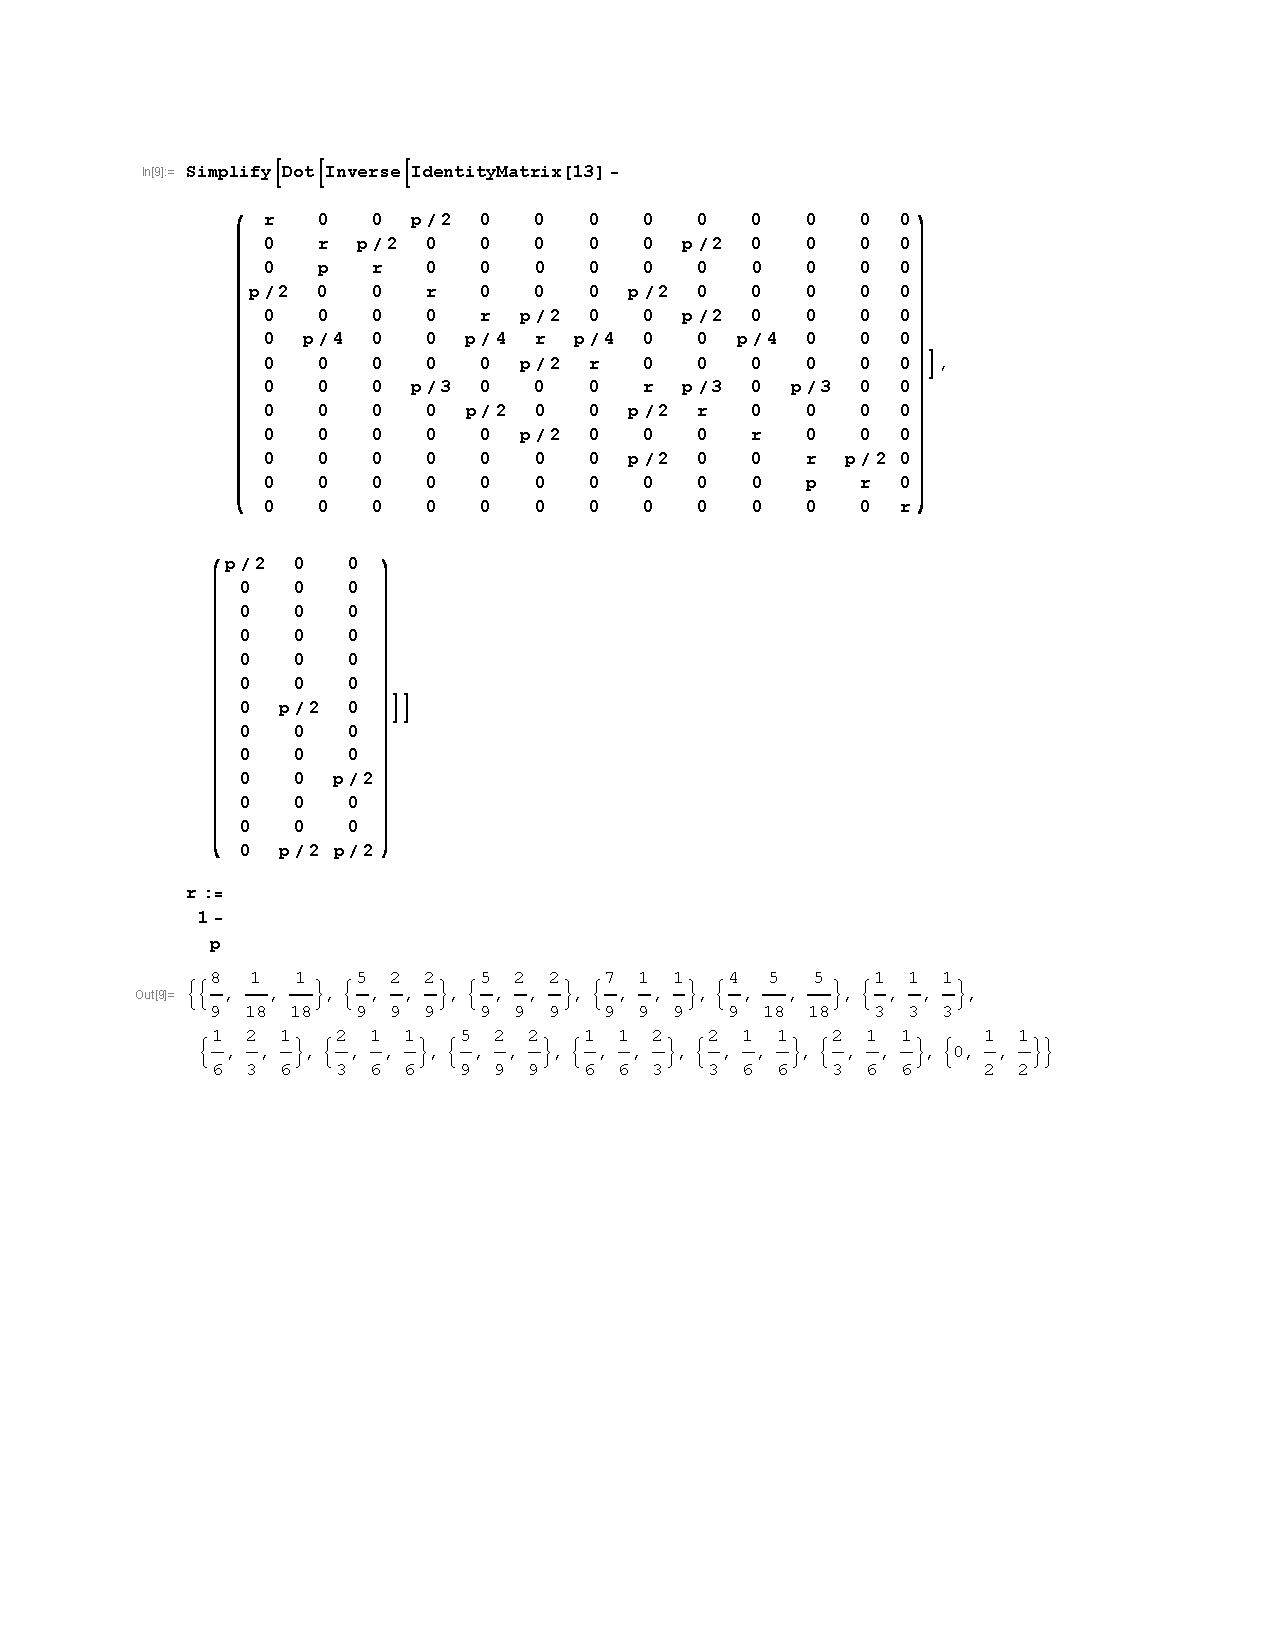
\includegraphics{Assignment3MathematicaPrintout}
\end{figure}
\begin{figure}
  \centering
  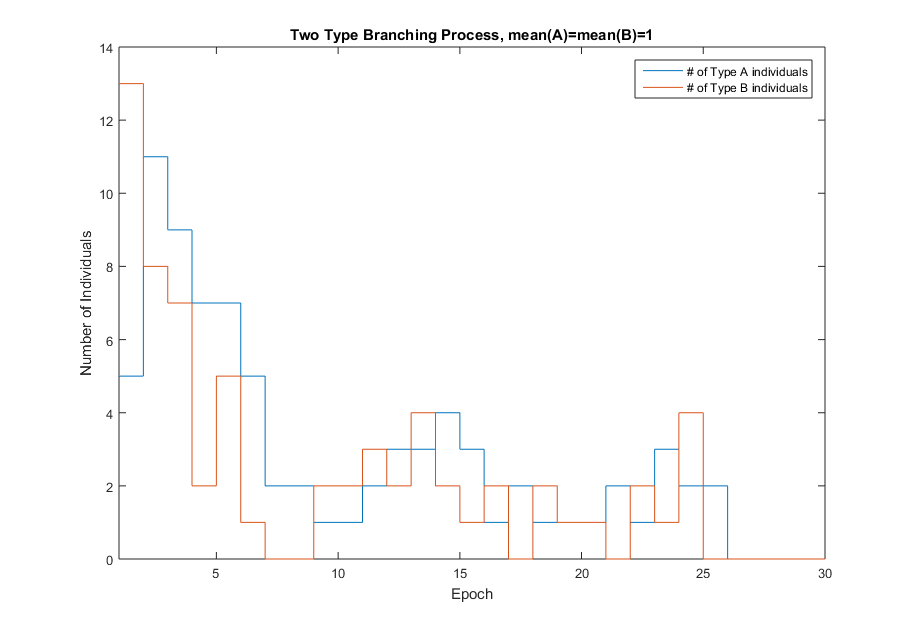
\includegraphics[width=0.75\textwidth]{branchingProcessDblExtinction}
\end{figure}
\begin{figure}
    \centering
    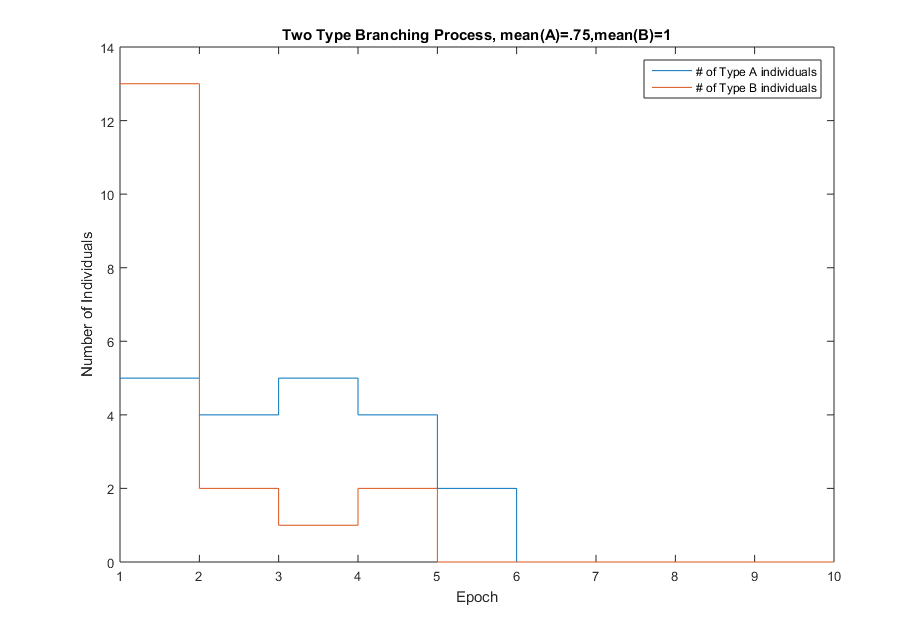
\includegraphics[width=0.75\textwidth]{branchingProcessDblExtinction2}
\end{figure}
\begin{figure}
    \centering
    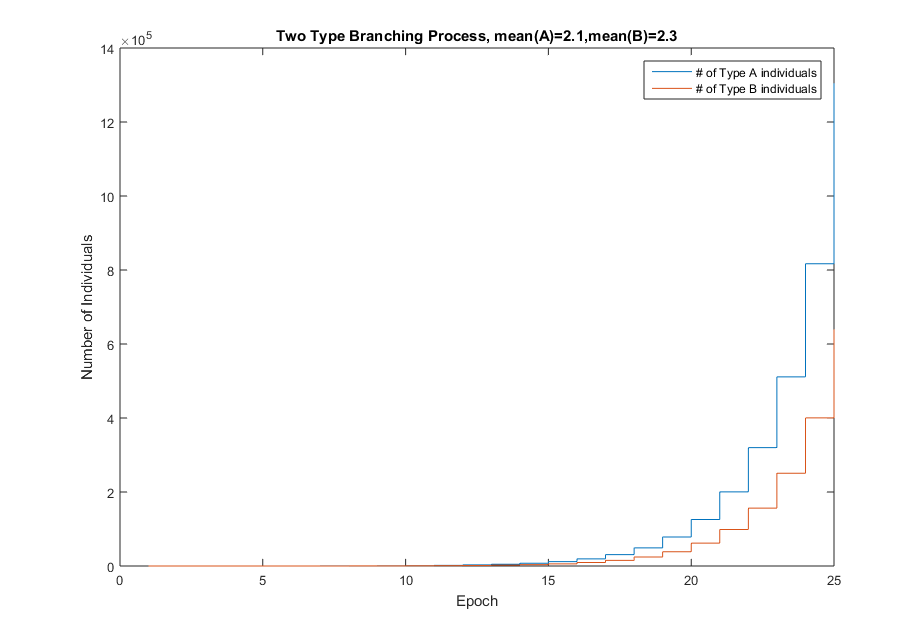
\includegraphics[width=0.75\textwidth]{branchingProcessUnlimitedGrowth}
\end{figure}
\begin{figure}
\centering
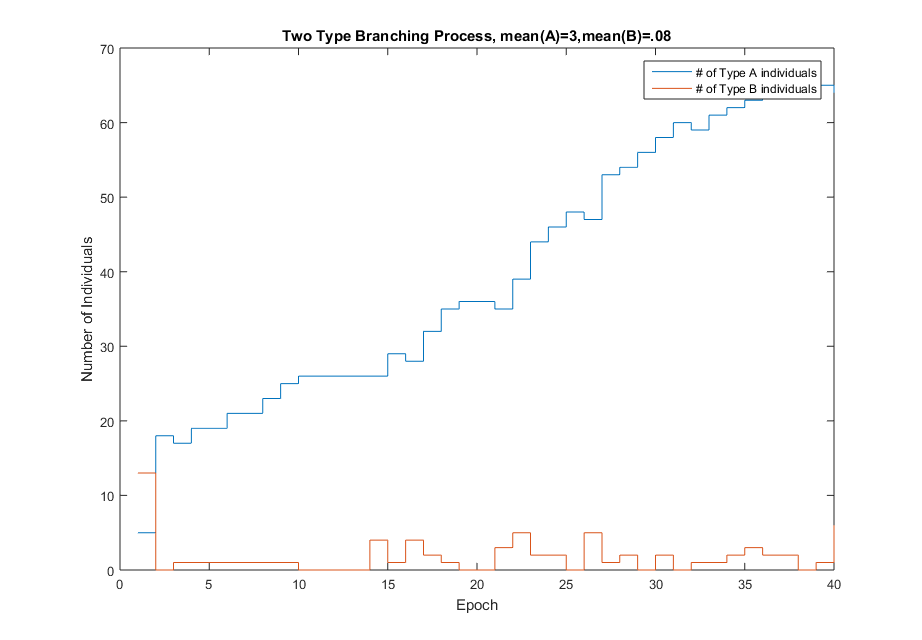
\includegraphics[width=0.75\textwidth]{branchingProcessOneFlourish}
\end{figure}
\begin{figure}
\centering
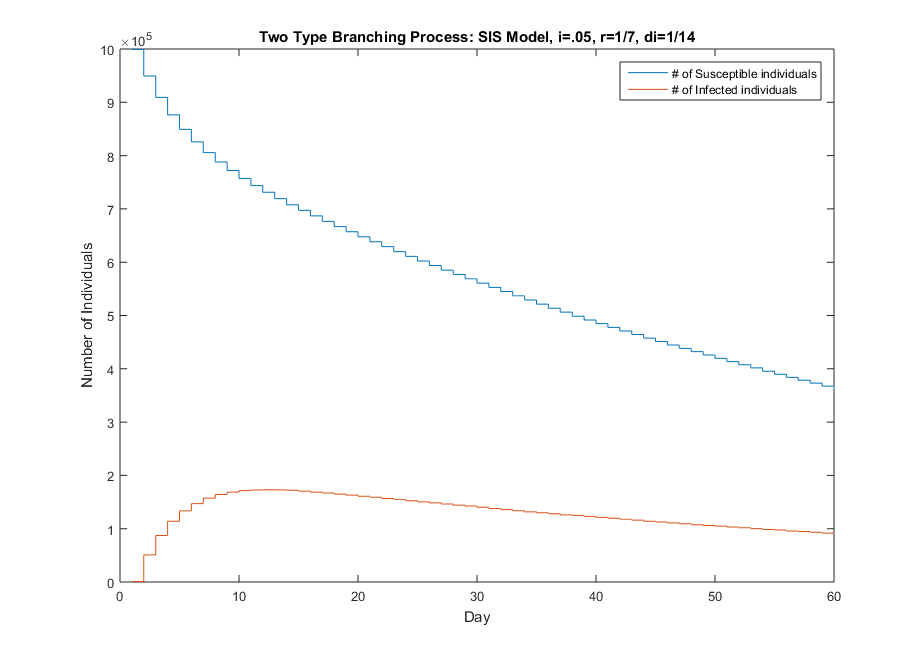
\includegraphics[width=0.75\textwidth]{branchingProcessSISModelSurvival}
\end{figure}
\begin{figure}
\centering
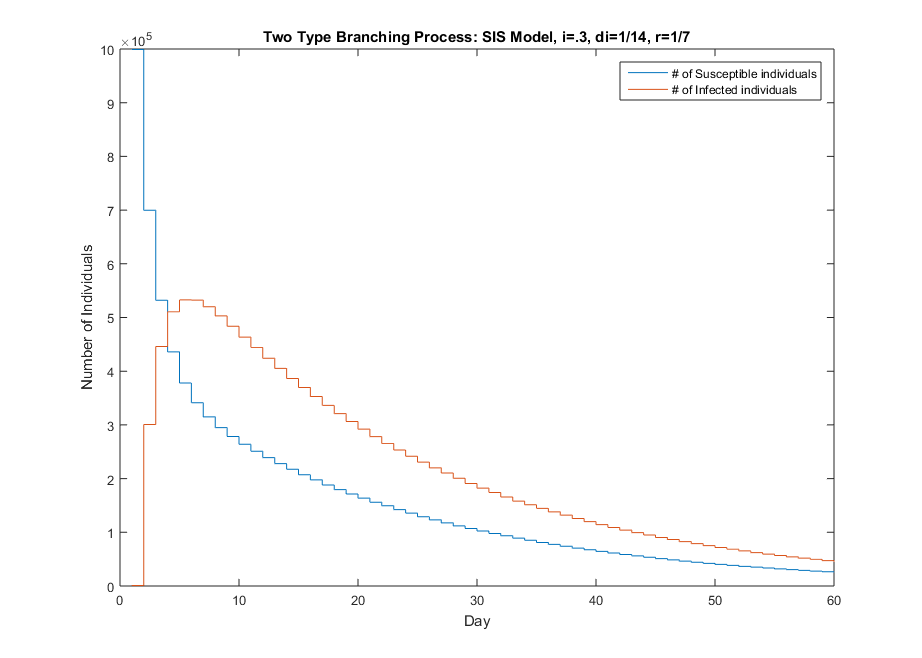
\includegraphics[width=0.75\textwidth]{branchingProcessSISModelNearDeath}
\end{figure}
\begin{figure}
\centering
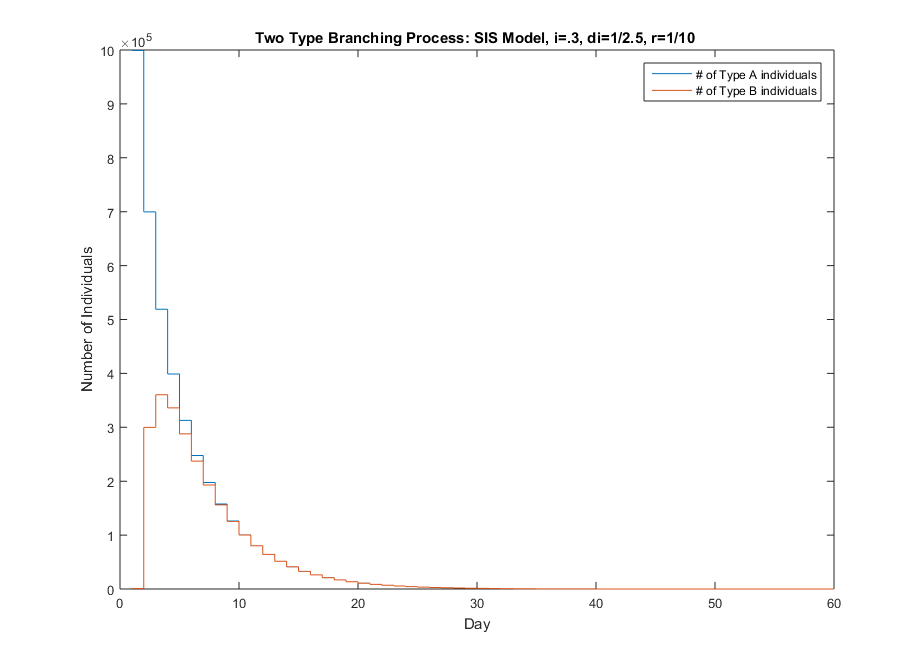
\includegraphics[width=0.75\textwidth]{branchingProcessSISModelDeath}
\end{figure}
\begin{figure}
\centering
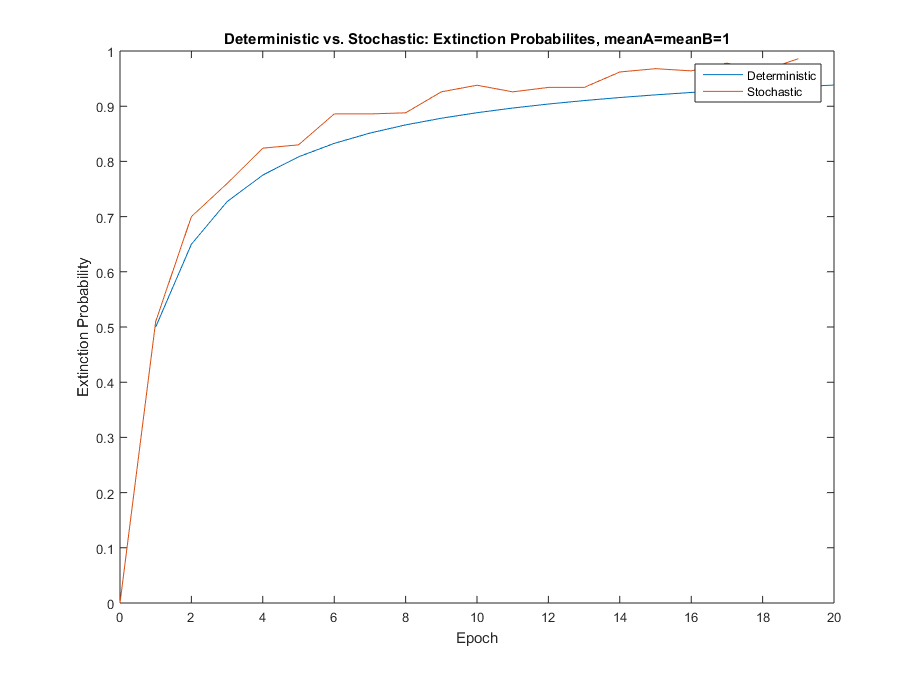
\includegraphics[width=0.75\textwidth]{extinctionprobmean1}
\end{figure}
\begin{figure}
\centering
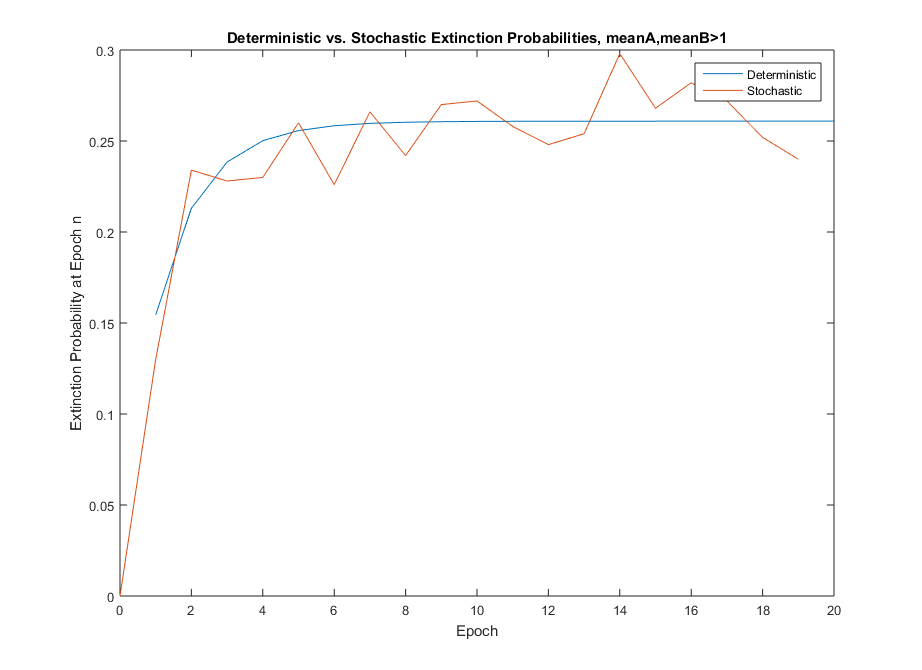
\includegraphics[width=0.75\textwidth]{extinctionprobmeanmore1}
\end{figure}
\begin{figure}
\centering
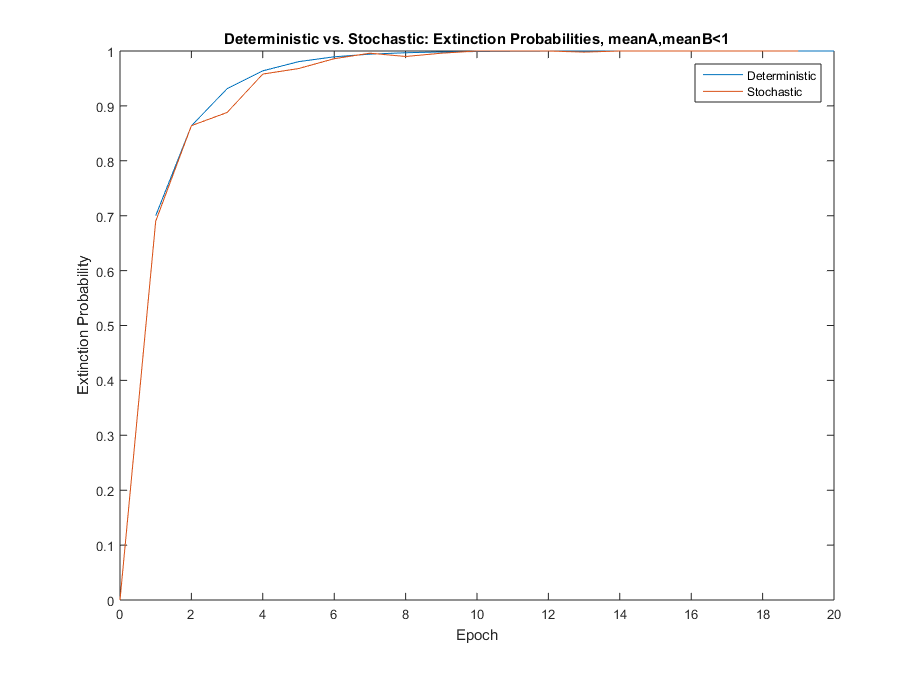
\includegraphics[width=0.75\textwidth]{extinctionprobmeanless1}
\end{figure}    
\end{section}
\end{document} 